\documentclass[12pt]{article}
%\usepackage{a4wide}
\usepackage[margin=2.5cm,a4paper]{geometry}
%\usepackage[latin1]{inputenc}
\usepackage{amsmath}
\usepackage{amsthm}
\usepackage{paralist}
\usepackage{bbm}
\usepackage{amssymb}
\usepackage{pdfpages}
\usepackage[T1]{fontenc}

\usepackage[pdftex,bookmarks,colorlinks,breaklinks,pdfpagelabels]{hyperref} 

\usepackage{epic,eepic,latexsym,verbatim}
%\usepackage{youngtab}
%\usepackage{bbm}
\newcommand{\ket}[1]{|#1\rangle}
\newcommand{\bra}[1]{\langle #1|}
\newcommand{\bracket}[2]{\langle #1|#2\rangle}
\newcommand{\ketbra}[1]{|#1\rangle\langle #1|}
\newcommand{\average}[1]{\langle #1\rangle}
\newcommand{\minus}{\!-\!}

\newcommand{\om}{\omega}
%\newcommand{\th}{\theta}
\newcommand{\rn}{\mathbb{R}^n}
\newcommand{\R}{\mathbb{R}}
\setlength{\parindent}{0pt}
\newtheorem{theorem}{Theorem}
\newcommand{\question}[2]{{\bf #1} {\em #2}\\}
\newcommand{\problem}[3]{{\bf #1} {\em #2}\\[5\lineskip]
{#3}}

\newcounter{dummy}
\setcounter{dummy}{0}
\newtheorem{p}{Exercise}[dummy]
\renewcommand\thep{\arabic{p}}
\setcounter{secnumdepth}{0}
\overfullrule=5pt

\author{Joseph M.\ Renes}
\title{Solutions to Baez and Muniain's \\\emph{Gauge Fields, Knots and Gravity}}
\begin{document}
\renewcommand{\abstractname}{\vspace{-\baselineskip}}


\hypersetup{pageanchor=true}

\maketitle

\begin{abstract}
Here are my solutions to some of the problems in \emph{Gauge Fields, Knots and Gravity}. 
At some point I also wrote up a few notes on the Lie derivative in the style of the book.\\

version 1.0 --- Importing original writeup of solutions and Lie derivative.
\end{abstract}

\pdfbookmark[1]{\contentsname}{Contents}
\tableofcontents



\newpage

\section{Part I}
%!TEX root = ../gfkg.tex
\subsection{Chapter 1}
\begin{p}
{Let $\vec{k}\in\R^3$ and lt $\omega=|\vec{k}|$. Fix $\vec{E}\in\mathbb{C}^3$ with 
$\vec{k}\cdot\vec{E}=0$ and $\vec{k}\times\vec{E}=i\omega\vec{E}$. Show that 
$\vec{\mathcal{E}}(t,\vec{x})=\vec{E}e^{-i(\omega t-\vec{k}\cdot\vec{x})}$ satisfies the
vacuum Maxwell equations.}
\end{p}
{...}



\subsection{Chapter 2}

\begin{p}
%{\bf 2} {\em 
Show that the two definitions of continuity are equivalent: 
 \begin{itemize}
\item Topological definition: $f$ is continuous if for any open $U\subset Y$, $f^{-1}(U)\subset X$ is also open
 \item $\epsilon-\delta$ definition: $f$ is continuous when for all $x$ and $\epsilon>0$, there exists a $\delta>0$ such that $||x-x'||<\delta$ implies $||f(x)-f(x')||<\epsilon$. 
\end{itemize}
\end{p}
{
 \begin{itemize}
\item[$\Rightarrow$] Pick $f(x)\in Y$ and $\epsilon>0$. Set $U=\{y:||y-f(x)||<\epsilon\}$, which is an open set . Thus $f^{-1}(U)$ is also an open set. This means that for all $x\in f^{-1}(U)$ all points sufficiently close to $x$ are also in $f^{-1}(U)$ or, put differently, for all $x$ there exists $\delta>0$ such that $N_\delta(x)=\{x':||x-x'||<\delta\}\subset f^{-1}(U)$. Thus, $f(x')\in U$ for all $x'\in N_\delta(x)$, which means there exists a $\delta>0$ such that $||x-x'||<\delta$ implies $||f(x)-f(x')||<\epsilon$

 \item[$\Leftarrow$] Pick any open $U$. Now we must show that $f^{-1}(U)$ is open. For any $f(x)\in U$ there exists $\delta>0$ such that $||x-x'||<\delta$ means $||f(x)-f(x')||<\epsilon$, so we can pick $\epsilon$ small enough to ensure that $\{f(x'):||f(x)-f(x')||<\epsilon\}\subset U$. Hence, for any point $x\in f^{-1}(U)$, points sufficiently close are also in $f^{-1}(U)$: $f^{-1}(U)$ is open. 
\end{itemize}
}

\begin{p}
Show that $S^n\subset \R^{n+1}$ with its induced topology is a manifold.
\end{p}
We need to check that the transition functions are smooth. This can be ensured by 
mapping each of the subsets of the sphere back into $\R^{n+1}$ and
applying the transition function there (it's the identity function there).


\begin{p}
Show that if $M$ is a manifold and $U$ is an open subset of $M$, then $U$ with its 
induced topology is a manifold.
\end{p}
{
The only thing one really needs to check is the smoothness of the transition functions
$\varphi_\alpha \circ \varphi_\beta^{-1}$. But this property is directly inherited from $M$,
since subsets of the form $U \cap S$ where $S$ is open in $M$ are themselves open
subsets of $M$.
}

\begin{p}
Given topological spaces $X$ and $Y$, we give $X\times Y$ the product topology in which a set is open if and only if it is a union of sets of the form $U\times V$,where $U$ is open in $X$ and $V$ is open in $Y$. Show that if $M$ is an $m$-dimensional manifold and $N$ is an $n$-dimensional manifold, $M \times  N$ is an $(m + n)$-dimensional manifold.
\end{p}
{...}
\begin{p}
Given topological spaces $X$ and $Y$, we give $X\times Y$ the disjoint union topology in which a set is open if and only if it is the union of an open subset of $X$ and an open subset of $Y$. Show that if $M$ and $N$ are $n$-dimensional manifolds the disjoint union $M \cup N$ is an $n$-dimensional manifold.
\end{p}
{...}




%!TEX root = ../gfkg.tex
\subsection{Chapter 3}
\begin{p}
{Show that $v+w$ and $gw\in \text{Vect}(M)$.}
\end{p}

$[v+w](f+g)=v(f+g)+w(f+g)=v(f)+w(f)+v(g)+w(g)=[v+w](f)+[v+w](g)$\\
$[v+w](\alpha f)=v(\alpha f)+w(\alpha f)=\alpha (v(f)+w(f))=\alpha[v+w](f)$\\
$[v+w](fg)=v(fg)+w(fg)=v(f)g+f v(g)+w(f)g+f w(g)=[v+w](f)g+f[v+w](g)$.\\

$[gw](f+h)=g\, w(f+h)=g(w(f)+w(h))=[gw](f)+[gw](h)$.\\
$[gw](\alpha f)=g\, w(\alpha f)=\alpha g\, w(f)=\alpha[gw](f)$.\\
$[gw](fh)=g\,w(fh)=g(w(f)h+fw(h))=g\,w(f)h+fg\,w(h)=[gw](f)\,h+f\,[gw](h)$.


\begin{p} Show that the following rules hold for all $v, w\in \text{Vect}(M)$ {\em and}
$f,g\in C^\infty(M)$: 1. $f(v+w)=fv+fw$, 2. $(f+g)v=fv+gv$, 3. $(fg)v=f(gv)$, 4. $1v=v$, where 1 denotes the constant function equal to 1 on all of $M$. This makes $\text{Vect}(M)$ 
a \emph{module} over $C^\infty(M)$.
\end{p}
$f(v+w)[g]=fv(g)+fw(g)$, so the first one holds. The remainder work exactly the same way:
apply both sides of the equation to a test function and show that they are equal.

\begin{p}
{Show that if $v^\mu\partial_\mu=0$ we must have $v^\mu=0$ for all $\mu$.}
\end{p}
Choose as test functions the coordinate functions $x^\mu$ so that $\partial_\mu x^\mu = 1$ for all
$\mu$, meaning $v=0$.

\begin{p}
{Let $v,w\in$ \emph{Vect($M$)}. Show that $v=w$ iff $v_p=w_p$ for all $p\in M$.}
\end{p}
If $v=w$ then $v_p=w_p$ since $v_p(f)=v(f)[p]=w(f)[p]=w_p$ for all $f$. If $v_p=w_p$, 
then $v(f)[p]=v_p(f)=w_p(f)=w(f)[p]$ for all $p\in M$ and $f\in C^\infty(M)$, so $v=w$.


\begin{p}
{Show that $T_p M$ is a vector space over the real numbers.}
\end{p}
... Need to show linearity, closedness, and existence of a zero.

\begin{p}
{Check that $\gamma'(t)\in T_{\gamma(t)}M$.}
\end{p}

$\gamma'(t)[f+g]=\frac{\rm d}{{\rm d}t}(f(\gamma(t))+g(\gamma(t)))=\gamma'(t)[f]+\gamma'(t)[g]$. Similarly
we get $\gamma'(t)[\alpha f]=\alpha \gamma'(t)[f]$. Finally, $\gamma'(t)[fg]=\frac{\rm d}{{\rm d}t}
(f(\gamma(t))g(\gamma(t)))=\gamma'(t)[f]g+f\gamma'(t)[g]$.

\begin{p}
Let $\phi: \R\rightarrow \R$ be given by $\phi(t)=e^t$. Let
$x$ be the usual coordinate function on $\R$. Show that $\phi^*x=e^x$.
\end{p}

The coordinate of the transformed point $\phi(p)$ is clearly $e^{x(p)}$, so $\phi^*x$ should be $e^x$. More
formally, $\phi^*x(p)=x(\phi(p))=x(e^{p})=e^{x(p)}$ so indeed $\phi^*x=e^x$.
%It's a little tricky to keep the notion of the coordinate function $x:M\rightarrow \R$ and its value $x(p)$ at the point $p$ distinct, and it will just get worse when looking at derivatives of $x$.\\

{\begin{p}
{Let $\phi:\R^2\rightarrow \R^2$ be a rotation counterclockwise
by an angle $\theta$. Let $x,y$ be the usual coordinate functions on $\R^2$. Show that
$\phi^*x=x\cos \theta-y\sin\theta$ and $\phi^*y=x\sin\theta+y\cos\theta$.}
\end{p}

Again $\phi^*x(p)=x(\phi(p))$, the $x$ coordinate of the rotated point. 
If $p$ is the point $(s,t)$, then 
$\phi(p)=(s',t')=(s\cos\theta-t\sin\theta,s\sin\theta+t\cos\theta)$. 
Thus $\phi^*x(p)=s\cos\theta-t\sin\theta=x(p)\cos\theta-y(p)\sin\theta$ and similarly for $\phi^*y$. 
Since the point $p$ is arbitrary, the desired result follows.

\begin{p}{$\phi:M\rightarrow N$ is smooth if $f\in C^\infty(N)$ implies $\phi^*f\in C^\infty(M)$. Show
that this definition is consistent with smooth functions $f:M\rightarrow\R$ and smooth
curves $\gamma:\R\rightarrow M$.}
\end{p}

A function $f:N\rightarrow\R$ is smooth if 
$f\circ\varphi^{-1}_\alpha:\R^n\rightarrow \R$ is smooth
for all $\alpha$. Pulling the function back by using $\phi$ makes a new smooth function $f':M\rightarrow 
\R$ where $f'=f\circ\phi$ since its smoothness is determined by
that of $(f\circ\phi)\circ(\varphi_\alpha\circ\phi)^{-1}=f\circ\varphi^{-1}_\alpha$ which is assumed to
be smooth. Any other coordinate system for $M$ would also produce a smooth result, since the 
different systems are related by smooth coordinate transformations.

\begin{p}{Prove that $(\phi\circ\gamma)'(t)=\phi_*(\gamma'(t))$}
\end{p}

$\phi_*(\gamma'(t))[f]=\gamma'(t)(\phi^*f)=\gamma'(t)(f\circ\phi)=\frac{\rm d}{{\rm d}t}(f\circ\phi)(\gamma(t))=\frac{\rm d}{{\rm d}t}f(\phi(\gamma(t)))=\frac{\rm d}{{\rm d}t}f((\phi\circ\gamma)(t))=(\phi\circ\gamma)'(t)[f]$

\begin{p}
 Show that the pushforward operation $\phi_*:T_pM\rightarrow T_{\phi(p)}N$ is linear.
 \end{p}

$\phi_*(v+w)[f]=(v+w)(\phi^*f)=v(\phi^*f_+w(\phi^*f)=\phi_*v[f]+\phi_*w[f]$ and similarly for scalars $\alpha$.

\begin{p}{Show that if $\phi:M\rightarrow N$
we can push forward a vector field $v$ on $M$ to obtain a vector field 
$\phi_*v$ on $N$ satisfying $(\phi_*v)_q=\phi_*(v_p)$ whenever $\phi(p)=q$.}
\end{p}

Since the vector fields can be specified pointwise, it suffices to consider a general point $p$. 
Now, $(\phi_*v)_q[f]=\phi_*v(f)[q]=v(f\circ\phi)[p]=v_p(\phi^*f)=\phi_*(v_p)[f]$.

\begin{p}
{Let $\phi:\R^2\rightarrow\R^2$ be rotation counterclockwise
by an angle $\theta$. Let $\partial_x,\partial_y$ be the coordinate vector fields on $\R^2$. 
Show that at any point of $\R^2$: $\phi_*\partial_x=(\cos\theta)\partial_x+(\sin\theta)\partial_y$
and $\phi_*\partial_y=-(\sin\theta)\partial_x+(\cos\theta)\partial_y$.}
\end{p}

Intuitively, this is just a rotation of the vectors, since they are tangent vectors to the coordinate paths
which are rotated by $\phi$. To make this more precise, consider $(\phi_*\partial_x)f=\partial_x(\phi^*f)=
\partial_x(f\circ\phi)$. Note that $\partial_x$ really means the derivative of the
function with respect to whatever quantity is in the first input; choosing the point $(x,y)$ as the input
makes this automatic. Then $\partial_x(f\circ\phi)(x,y)=\partial_uf \cdot \partial_x u+\partial_v f\cdot \partial_x v$, where $(u,v)=(x\cos\theta-y\sin\theta,x\sin\theta+y\cos\theta)=\phi(x,y)$. We then obtain
$(\phi_*\partial_x)f=(\cos\theta)\partial_u f+(\sin\theta)\partial_vf$. Since $u$ is the first input to $f$, $\partial_u$ is
the same as $\partial_x$ in the rotated space, and similarly for $v$ and $y$. This gives us
$\phi_*\partial_x=(\cos\theta)\partial_x+(\sin\theta)\partial_y$; the same argument works for $\phi_*\partial_y$.

\begin{p}{Let $v$ be the vector field $x^2\partial_x+y\partial_y$ on $\R^2$. Calculate 
the integral curves $\gamma(t)$ and see which ones are defined for all $t$.}
\end{p}

We start by making up a representation. $\gamma'(t)[f]=\frac{\rm d}{{\rm d}t}f(\gamma(t))
=\partial_\mu f\frac{{\rm d}\gamma^\mu}{{\rm d}t}$, so $\gamma'(t)=
\frac{{\rm d}\gamma^\mu}{{\rm d}t}\partial_\mu$. 
If $\gamma(t)=(x(t),y(t))$, then $\gamma'(t)=\dot{x}(t)\partial_x+\dot{y}(t)\partial_y$. 
Then $\dot{x}=x^2$ and $\dot{y}=y$. The solution is $\gamma(t)=(x(0)/(1-x(0)t),y(0)e^t)$, which
is finite for finite $t$ provided $1-x(0)t\neq 0$. Thus, only the curves with $x(0)=0$ are defined for all
$t$.

\begin{p}{Show that $\phi_0$ is the identity map id:$X\rightarrow X$, and that for all $s,t\in\R$ we have $\phi_t\circ\phi_s=\phi_{t+s}$.}
\end{p}

The point $p$ is translated to the point $\gamma(t)$ along the integral curve $\gamma$ of $v$ with $p$
as the initial point. Since $\gamma(0)=p$, $\phi_0(p)=p$. Moreover, as the integral curve is the solution
to a first-order differential equation, the solutions are unique and the curves don't intersect. If we move
apply $\phi_t\circ\phi_s$ to $p$ we are first moving the point $p=\gamma(0)$ to $\gamma(s)$ and then using
this point as the new intial value for the integral curve so that we can move it to $\widetilde{\gamma}(t)$. But 
the curves are unique and any point on the curve defines a boundary condition which together with
the differential equation, yields the curve. Thus, $\gamma$ and $\widetilde{\gamma}$ are the same curve
with the same parameterization (except for the offset).

\begin{p}
{Consider the normalized vector fields in the $r$ and $\theta$ direction on the plane in polar coordinates (not defined at the origin):
\[
v=\frac{x\partial_x+y\partial_y}{\sqrt{x^2+y^2}},\qquad w=\frac{x\partial_y-y\partial_x}{\sqrt{x^2+y^2}}
\]
Calculate $[v,w]$}.
\end{p}

Let's put this into component notation first. Define $\bar{r}=1/\sqrt{x^2+y^2}$,
$x_0=x$, and $x_1=y$. Then $v=\bar{r}x^k\partial_k$ while $w=\bar{r}\epsilon^j_i x^i\partial_j$, for $\epsilon^j_i$ the antisymmetric symbol/tensor. Before getting started, note that $\partial_j\bar{r}=-x_j\bar{r}^3$ (watch out for the lower index!). Now
\begin{eqnarray*}
[v,w]&=&vw-wv=\bar{r}x^k\partial_k(\bar{r}\epsilon^j_ix^i\partial_j)-
\bar{r}\epsilon^j_ix^i\partial_j(\bar{r}x^k\partial_k)\\
&=&\bar{r}^2\epsilon^j_ix^k\left(\delta_k^i\partial_j+x^i\partial_k\partial_j-\bar{r}^2x_k x^i\partial_j\right)-\bar{r}^2\epsilon^j_i x^i\left(\partial_j+x^k\partial_j\partial_k-\bar{r}^2 x_j x^k\partial_k\right)\\
&=&-\bar{r}^4x^kx_k\epsilon^j_i x^i\partial_j=-\bar{r}^2\epsilon^j_i x^i\partial_j=-\frac{x\partial_y-y\partial_x}{x^2+y^2}=-\frac{w}{r},
\end{eqnarray*}
since $[\partial_i,\partial_j]=0$ and $\epsilon^j_ix^ix_j=0$.

\begin{p}{Check that $[v,w](f)(p)=\frac{\partial^2}{\partial t \partial s}\left[
f(\psi_s(\phi_t(p)))-f(\phi_t(\psi_s(p)))\right]_{s=t=0}$}
\end{p}

Start with $(vf)(p)=\frac{d}{dt}f(\phi_t(p))|_{t=0}$ and
$(wf)(p)=\frac{d}{ds}f(\psi_s(p))|_{s=0}$. 
Then we have $(vwf)(p)=v(wf)(p)=\frac{d}{dt}wf(\phi_t(p))|_{t=0}=\frac{\partial^2}{\partial t\partial s}f(\psi_s(\phi_t(p)))|_{s=t=0}$. Note that $wf$ means take $f$ and displace its input a little bit, and evaluate the derivative at zero
displacement. In the compound expression, the input to $f$ is $\phi_t(p)$, so $\psi_s$ ends up first inside $f$ in the final expression. Alternatively, we could work from inside-out: $v(wf)(p)=v\left(\frac{d}{dt}f(\psi_s(\cdot))|_{s=0}\right)(p)=\frac{\partial^2}{\partial t\partial s}f(\psi_s(\phi_t(p)))|_{s=t=0}.$
Similarly, $(wvf)(p)=\frac{\partial^2}{\partial t\partial s}f(\phi_t(\psi_s(p)))|_{s=t=0}$, so the expression for the commutator holds.

\begin{p}{Show that for all vector fields $u, v, w$ on a manifold, and all real numbers $\alpha$ and $\beta$, we have:
\begin{enumerate}
\item $[v,w]=-[w,v]$
\item $[u,\alpha v+\beta w]=\alpha[u,v]+\beta[u,w]$
\item The {\bf Jacobi identity}: $[u,[v,w]]+[v,[w,u]]+[w,[u,v]]=0$
\end{enumerate}}
\end{p}
\begin{enumerate}
\item $[u,v]=uv-vu=-(vu-uv)=-[v,u]$
\item $[u,\alpha v+\beta w]=u(\alpha v+\beta w)-(\alpha v+\beta w)u=\alpha[u,v]+\beta[u,w]$
\item $[u,[v,w]]=u(vw-wv)-(vw-wv)u$, so $[u,[v,w]]+[v,[w,u]]+[w,[u,v]]=
u(vw-wv)-(vw-wv)u+v(wu-uw)-(wu-uw)v+w(uv-vu)-(uv-vu)w=0$
\end{enumerate}



%!TEX root = ../gfkg.tex
\subsection{Chapter 4}
\begin{p}
{Show that $\omega+\mu$ and $f\omega$ are really 1-forms, i.e.\ show linearity over $C^\infty(M)$.}
\end{p}

That $\omega$ and $\mu$ are 1-forms means they are (separately) linear over $C^\infty(M)$. So $[\omega+\mu](v+w)=
\omega(v+w)+\mu(v+w)=\omega(v)+\omega(w)+\mu(v)+\mu(w)=[\omega+\mu](v)+[\omega+\mu](w)$. $f\omega$ is just
multiplication by $f$ of the result of applying $\omega$, so $[f\omega](v+w)=f\omega(v+w)=f\omega(v)+f\omega(w)$.

\begin{p}{Show that $\Omega^1(M)$ is a module over $C^\infty(M)$.}
\end{p}

There are four conditions to check. Let $f,g\in C^\infty(M)$ and $\omega,\mu\in C^\infty(M)$. The first condition
is $f(\omega+\mu)=f\omega+f\mu$, which is true by applying each side of the equation to a test vector $v$ and
using the previous exercise to show the two resulting expressions are equal. Same for the conditions $(f+g)\omega=f\omega+g\omega$,
$(fg)\omega=f(g\omega)$, and $1\omega=omega$. Basically the point is that by applying the 1-forms to test vectors, everything
turns into functions and the equality of the different expressions follows immediately.\\

\begin{p}
{Show that $d(f+g)=df+dg, d(\alpha f)=\alpha\, df, (f+g)dh=f\,dh+g\,dh$, and $d(fg)=f(dg)+g(df)$ for any
$f,g,h\in C^\infty(M)$ and any $\alpha\in \R$.}
\end{p}

The differential map $d$ is defined by $df(v)=vf$. Applying this definition to the first equation, we obtain $d(f+g)v=v(f+g)=vf+vg=df(v)+dg(v)=[df+dg](v)$ as intended. Similarly, $d(\alpha f)(v)=v(\alpha f)=\alpha vf=\alpha df(v)$
and $(f+g)dh(v)=(f+g)vh=f\,vh+g\,vh=[f\,dh+g\,dh](v)$. For the last condition, compute $d(fg)(v)=v(fg).$ By the definition
of $v$ as a vector field, $v(fg)=gv(f)+fv(g)$, so we obtain $d(fg)(v)=[f(dg)+g(df)](v)$.\\

\begin{p}{Suppose $f(x^1,\dots,x^n)$ is a function on $\R^n$. Show that $df=\partial_\mu f\,dx^\mu$.}
\end{p}

Consider an arbitrary vector field $v=v^\nu \partial_\nu$. Then $df(v)=vf=v^\nu \partial_\nu f$. On the other hand, $(\partial_\mu f\,dx^\mu)v=\partial_\mu f\, vx^\mu=\partial_\mu f\, v^\nu\partial_\nu x^\mu=\partial_\mu f\, v^\nu \delta_\nu^\mu=v^\nu \partial_\nu f$. 
So $df=\partial_\mu f\,dx^\mu$ as intended.

{\begin{p}{Show that the 1-forms $\{dx^\mu\}$ are linearly independent.}
\end{p}

Suppose $\omega=\omega_\mu\,dx^\mu=0$. Then $\omega(\partial_\nu)=\omega_\mu\,dx^\mu(\partial_\nu)=\omega_\mu \partial_\nu x^\mu
=\omega_\nu=0$.

\begin{p}{Show that $\omega(v)(p)$ really depends only on $v_p$, not on 
the values of $v$ at other points. Also, show that a 1-form is determined by its values at points.
In other words, if $\omega, \nu$ are two 1-forms on $M$ with $\omega_p=\nu_p$ for 
every point $p\in M$, then $\omega=\nu$. }
\end{p}

Suppose $w$ is a vector field for which $w_p=0$ but generally $w_q\neq 0$. By linearity, $\omega(v+w)=\omega(v)+\omega(w)$. 
Specializing to the point $p$, we have $\omega(v+w)(p)=\omega(v)(p)+\omega(w)(p)=\omega_p(v_p)+\omega_p(w_p)$. But
since $w_p=0$, the latter term is zero, and $\omega(v+w)(p)=\omega(v)(p)$. This means we can change the field $v$ at points
distinct from $p$ and still obtain the same action by $omega$ at the desired point. Note that this works due to the linearity of the
map $\omega$.\\

Since we can ``decompose'' the field $v$ into tangent vectors $v_p$ at each point $p\in M$, (excercise 10), we have 
$\omega_p(v_p)=\nu_p(v_p) = \omega(v)(p)=\nu(v)(p)$. This has to hold for any $v$ and all $p$, so $\omega=\nu$.\\

\begin{p}{Show that the dual of the identity map on a vector space $V$ is the identity map on $V^*$. Suppose
that we have linear maps $f:V\rightarrow W$ and $g:W\rightarrow X$. Show that $(gf)^*=f^*g^*$. }
\end{p}

The dual of a function $f$ is defined by $(f^*\omega)(v)=\omega(f(v))$. So if $f$ is the identity, then $(f^*\omega)(v)=\omega(v)$,
meaning that $f^*$ must be the identity as well. 
Now we find $[(gf)^*\omega](v)=\omega(g(f(v)))=[g^*\omega](f(v))=[f^*g^*\omega](v)$,
so  $(gf)^*=f^*g^*$.

\begin{p}{Show that the pullback defined by the equation $(\phi^*\omega)_p=\phi^*(\omega_q)$, where $\phi(p)=q$,
really exists and is unique.}
\end{p}

Start with  $(\phi^*\omega)_p(v_p)=\phi^*\omega(v)(p)=\omega(\phi_*v)(\phi(p))=\omega(\phi_*v)(q)$. The other 
side of the equation gives $\phi^*(\omega_q)v_q=\omega_q(\phi_* v_q)$, the same. Uniqueness follows from linearity: if there were
two possible outputs, we could consider their difference. By linearity this would be the result of applying the map to the difference of the
fixed input, which is zero. But the output of zero is zero, so the two possible outputs are equal.\\

\begin{p}{Let $\phi:\R\rightarrow \R$ be given by $\phi(t)=\sin t$. Let $dx$ be the usual
1-form on $\R$. Show that $\phi^*dx=\cos t\,dt$.}
\end{p}

$\phi^*(df)=d(\phi^*f)$ since the exterior derivative is natural. Thus $\phi^*(df)=d(\sin t)=\cos t\,dt$.

\begin{p}{Let $\phi:\R^2\rightarrow \R^2$ denote rotation counterclockwise by the 
angle $\theta$. Let $dx, dy$ be the usual basis of 1-forms on $\R^2$. Show that $\phi^*dx=\cos\theta\,dx-\sin\theta\,dy$
and $\phi^*dy=\sin\theta\,dx+\cos\theta\,dy$. }
\end{p}

$\phi^*dx=d(\phi^*x)=d(x\cos\theta-y\sin\theta)=\cos\theta\,dx-\sin\theta\,dy$. Similarly for $\phi^*dy$. 

\begin{p}{Show that the coordinate 1-forms $dx^\mu$ really are the differentials of the local coordinates $x^\mu$ on $U$.}
\end{p}

Technically, $x^\mu$ is the local coordinate on $\R^n$ which picks out the $\mu$th component. When speaking
of $x^\mu$ on $U$, we really mean $\phi^*x^\mu$, where $\phi$ is the map from $U$ to $\R^n$. Thus
$dx^\mu$ is really $d(\phi^*x^\mu)=\phi^*dx^\mu$, so the sloppiness of the notation doesn't injure the relationship
between functions and 1-forms.

\begin{p}{Show that $dx'^\nu=\frac{\partial x'^\nu}{\partial x^\mu}dx^\mu$. Show that for any 1-form $\omega$ on $\R^n$,
writing $\om=\om_\mu dx^\mu=\om'_\nu dx'^\nu$, the components $\omega'_\nu$ are related to the components $\omega_\mu$ by
$\omega'_\nu=\frac{\partial x^\mu}{\partial x'^\nu}\om_\mu$.}
\end{p}

For the first equation, apply both sides to the partial $\partial_\alpha$: $dx'^\nu(\partial_\alpha)=
\partial_\alpha(x'^\nu)$ and $\frac{\partial x'^\nu}{\partial x^\mu}dx^\mu(\partial_\alpha)=
\frac{\partial x'^\nu}{\partial x^\mu}\partial_\alpha(x^\mu)=
\frac{\partial x'^\nu}{\partial x^\mu}\delta^\mu_\alpha=\frac{\partial x'^\nu}{\partial x^\alpha}=
\partial_\alpha(x'^\nu)$. For the second, use the same trick. Apply $\om$ to 
$\frac{\partial}{\partial x'^\alpha}$. The left expression gives $\om_\mu dx^\mu(\frac{\partial}{\partial x'^\alpha})=
\om_\mu\frac{\partial x^\mu}{\partial x'^\alpha}$, while the right expression gives $\om'_\alpha$.\\

\begin{p}{Show that $\phi^*(dx'^\nu)=\frac{\partial x'^\nu}{\partial x^\mu}dx^\mu$.}
\end{p}

$\phi^*(dx'^\nu)\partial_\mu=d(\phi^*x'^\nu)\partial_\mu=\partial_\mu(\phi^* x'^\nu)=\frac{\partial x'^\nu}{\partial x^\mu}$.

\begin{p}{Let $e_\mu=T^\nu_\mu\partial_\nu$, where $\partial_\nu$ are the coordinate vector fields associated to local coordinates on
an open set $U$ and $T^\nu_\mu$ are functions on $U$. Show that the vector fields $e_\mu$ are a basis of vector fields on $U$ iff for 
each $p\in U$ the matrix $T^\nu_\mu(p)$ is invertible.}
\end{p}

\begin{itemize}
\item[$\Rightarrow$] The matrix $T^\nu_\mu(p)$ is invertible, so det$T\neq 0$, meaning the $e_u$ are linearly independent at $p$ and thus 
form a basis at $p$. Since this works for all $p$, the vector fields $e_\mu$ are a basis. 
\item[$\Leftarrow$] Try to expand an arbitrary $\om$ in terms of the $e_\mu$: $\om=\om^\mu e_\mu$. We can also express
$\om$ in terms of the $\partial_\nu$ as $\om=\om'^\nu\partial_\nu$, with $\om'^\nu= T^\nu_\mu \om^\mu$. If $T$ were not invertible, 
we would not be able to construct the $\om^\mu$ from the $\om'^\nu$ (which are the ones guaranteed to exist), so $e_\mu$ wouldn't be 
a basis. Since it is a basis, $T$ must be invertible. 
\end{itemize}

\begin{p}{Use the previous exercise to show that the dual basis exists and is unique}
\end{p}

Let $f^\mu$ be the putative dual basis to the $e_\nu$. Then $f^\mu(e_\nu)=\delta^\mu_\nu=T^\lambda_\nu f^\mu\partial_\lambda$.
Now suppose $f^\mu=S^\mu_\lambda dx^\lambda$. Inserting into the previous equation we obtain $T^\lambda_\nu S^\mu_\lambda=\delta^\mu_\nu$, so $S$ is the inverse of $T$. Since $T$ is invertible, the $f^\mu$ are well-defined and unique.

\begin{p}{Let $e_\mu$ be a basis of vector fields on $U$ and let $f^\mu$ be the dual basis of 1-forms. Let $e'_\mu=T^\nu_\mu e_\nu$
be another basis of vector fields, and let $f'^\mu$ be the corresponding dual basis of 1-forms. Show that $f'^\mu=(T^{-1})^\mu_\nu f^\nu$. Show
that if $v=v^\mu e_\mu=v'^\mu e'_\mu$, then $v'^\mu=(T^{-1})^\mu_\nu v^\nu$ and that if
$\om=\om_\mu f^\mu=\om'_\mu f'^\mu$ then $\om'_\mu=T^\nu_\mu \om_\nu$.}
\end{p}

This is where the ``historical'' definitions of co- and contra-variant come from, specifying whether something transforms like the components
of a vector or like the basis vectors themselves. (Vectors, being susceptible to pushforward, are covariant. 1-forms are contravariant, but the components of a vector are also contravariant, while the components of 1-forms are covariant.) For $f'^\mu$, apply it to $e'_\nu$:
$f'^\mu(e'_\nu)=\delta^\mu_\nu$. Using the definition of $e'_\nu$, $\delta^\mu_\nu=T_\nu^\lambda f'^\mu(e_\lambda)$. 
This works if $f'^\mu=(T^{-1})^\mu_\nu f^\nu$. All this can be done more easily in matrix notation. For the next case, let $\mathbf{v}$ be the 
ordered set of $v^\mu$ and likewise $\mathbf{e}$ the set of $e_\mu$. Then $v=\mathbf{v}\cdot\mathbf{e}$. Meanwhile, $\mathbf{e}'=T\mathbf{e}$, so clearly we're going to need $\mathbf{v}'=(T^{-1})^T\mathbf{v}$ so that 
$\mathbf{v}'\cdot\mathbf{e}'=\mathbf{v}T^{-1}T\mathbf{e}=v$. Thus, we predict that $v'^\mu=(T^{-1})^\mu_\nu v^\nu$, using
the inverse and transposed $T$ as given in the definition of $e'_\mu$. Similarly $\om=\mathbf{\om}\cdot\mathbf{f}$, so 
$\om'_\mu=T^\nu_\mu \om_\nu$.

\begin{p}{Show that $u\wedge v\wedge w={\rm det}\left(\begin{array}{ccc} u_x & u_y & u_z \\
v_x & v_y & v_z\\ w_x & w_y & w_z\end{array}\right)\,dx\wedge dy\wedge dz$. Compare this to $\vec{u}\cdot(\vec{v}\times\vec{w})$.}
\end{p}

...algebra

\begin{p}{Show that if $a,b,c,d$ are four 1-forms in a 3-dimensional space, then $a\wedge b\wedge c\wedge d=0$.}
\end{p}

Since there are only three linearly independent 1-forms in this space, the 4-fold wedge product will always contain two of the basis
elements twice, which by antisymmetry, means the entire expression must be zero.

\begin{p}{Describe $\bigwedge V$ if $V$ is 1-,2-,3-, or 4-dimensional.}
\end{p}

1-dimensional: scalars and vectors. 2-dimensional: scalars, vectors, and areas. 3-dimensional: scalars, vectors, areas, and volumes. 4-dimensional:
all the previous, plus 4-volumes.

\begin{p}{Let $V$ be an n-dimensional vector space. Show that $\bigwedge^{\!p} V$ is empty for $p>n$ and that for $0\leq p\leq n$ the dimension of $\bigwedge^{\!p} V$ is $n!/p!(n-p)!$.}
\end{p}

As in exercise 42, elements of $\bigwedge^{\!p} V$ are wedge products of $p$ different terms, but since there are only $n$ independent possibilities,
$\bigwedge^{\!p} V$ is empty for $p>n$. Wedging $p$ different terms for $p\leq n$ can be done in $\binom{n}{p}$ ways since by antisymmetry 
the order of the terms can only affect the sign of the result.

\begin{p}
{Show that $\bigwedge V=\bigoplus_p \bigwedge^{\!p} V$.}
\end{p}

Since we've defined $\bigwedge V$ formally, as the linear space of wedge products of elements of $V$, we then immediately have
that the different sectors corresponding to different number of wedgings $p$ are disjoint. Thus we can treat these 
completely independently from one another and form $n$-tuples containing entries from each sector. This will be an element of
$\bigwedge V$ since adding elements of distinct grade is also purely formal and can always be resolved into the various
graded components. Thus, $\bigwedge V=\bigoplus_p \bigwedge^{\!p} V$.

\begin{p}{Given a vector space $V$, show that $\bigwedge V$ is a graded commutative or supercommutative algebra;
that is, if $\om\in \bigwedge^{\!p}V$ and $\mu\in\bigwedge^{\!q}V$, then $\om\wedge\mu=(-1)^{pq}\mu\wedge\om$.}
\end{p}

This is essentially just a counting argument. $\om$ is the wedge of $p$ things, $\mu$ $q$. So to invert the order of wedging
them together means transporting $p$ elements of $V$ past $q$ elements of $V$, each time picking up a minus one.

\begin{p}{Show that differential forms are contravariant. That is, show that if $\phi:M\rightarrow N$ is a map from the manifold
$M$ to the manifold $N$, there is a unique pullback map $\phi^*:\Omega(N)\rightarrow\Omega(M)$ agreeing with the usual pullback 
on 0-forms (functions) and 1-forms, satisfying $\phi^*(\alpha\om)=\alpha\phi^*\om$, $\phi^*(\om+\mu)=\phi^*\om+\phi^*\mu$ and
$\phi^*(\om\wedge \mu)=\phi^*\om\wedge\phi^*\mu$, for all $\om,\mu\in\Omega(N)$ and $\alpha\in\R$.}
\end{p}

I take the three conditions to almost be the definition of the map. For a general $\om$, resolve it into a linear combination of 
graded components using an arbitrary basis of 1-forms to generate the $p$-forms. The by condition two the pullback applies to each
term separately. By condition one the coefficients of each term don't interfere with the pullback. Finally, by condition three we apply the pullback
to each of the 1-forms making up the basis $p$-forms, so the map is well-defined. Its unique because the pullback applied to 1-forms and 
functions is unique.

\begin{p}{Compare the transformation properties of 1-forms and 2-forms on $\R^3$ under parity. That is, let $P:\R^3\rightarrow\R^3$ be the map $P(x,y,z)=(-x,-y,-z)$, known as the `parity transformation'. 
Note that $P$ maps right-handed bases to left-handed bases and vice versa. Compute $\phi^*\om$ when $\om$ is the 1-form
$\om_\mu dx^\mu$ and when it is the 2-form $\frac{1}{2}\omega_{\mu,\nu} dx^\mu\wedge dx^\nu$.}
\end{p}

If prime variables refer to the output space, for instance $x'=-x$, the 
essential point is that $\phi^*(dx'^\mu)=d(\phi^* x'^\mu)=d(-x^\mu)=-dx^\mu$. Thus 
$\phi^*\om^{(1)}=-\om$ and $\phi^*\om^{(2)}=\om^{(2)}$.

\begin{p}{Show that on $\rn$ the exterior derivative of any 1-form is given by $d(\om_\mu dx^\mu)=\partial_\nu\om_\mu dx^\nu\wedge dx^\mu$.}
\end{p}

$d(\om_\mu dx^\mu)=d\om_\mu\wedge dx^\mu=\partial_\nu\om_\mu dx^\nu\wedge dx^\mu$.




\subsection{Chapter 5}

\begin{p}{Show that any 2-form $F$ on $\R\times S$ can be uniquely expressed as $B+E\wedge dt$ in 
such a way that for any local coordinates $x^i$ on $S$ we have 
$E=E_i dx^i$ and $B=\frac{1}{2}B_{ij} dx^i\wedge dx^j$.}
\end{p}

For some patch $U\subset S$, we can use the local coordinates $x^i$ along with $t\in\R$ to define an
element of $\R^{n+1}$. Any 2-form $F$ can be written as $F=F_{\alpha\beta} dx^\alpha\wedge dx^\beta$ where the summation
runs over $0\dots n$ and $x^0=t$. We can also express this as $F=F_{0i}dt\wedge dx^i+F_{i0}dx^i\wedge dt+F_{ij}dx^i\wedge dx^j$. 
But then by 
antisymmetry of the wedge product, we might as well have $F_{i0}=-F_{0i}$. Then defining $E_i=2F_{0i}$ we have
$F=E_i dx^i\wedge dt+F_{ij}dx^i\wedge dx^j$. With $B_{ij}=2F_{ij}$ we obtain $F=E\wedge dt+B$. This decomposition is unique 
because if it were true using different functions $E'_i$ and $B'_{ij}$, then their difference would be zero.

\begin{p}{Show that for any form $\om$ on $\R\times S$ there is a unique way to write $d\om=dt\wedge\partial_t\om+d_S\om$
such that for any local coordinates $x^i$ on $S$, writing $t=x^0$, we have $d_S\om=\partial_i \om_I dx^i\wedge dx^I$ and
$dt\wedge \partial_t\om=\partial_0\om_I dx^0\wedge dx^I$.}
\end{p}

First write $\om=\om_I dx^I$ for $I$ a multi-index of length $p$ (i.e. a $p$-tuple whose entries range over $0\dots n$, where
$n$ is the dimension of $S$). Then $d_S\om=\partial_i \om_I dx^i\wedge dx^I$ and $\partial_t\om=\partial_0\om_I$. Again, uniqueness
follows from linearity: if there were two possibilities, their difference would be zero by the linearity of $d$, implying their equality.

\begin{p}{Use the nondegeneracy of the metric to show that the map from $V$ to $V^*$ given by $v\mapsto g(v,\cdot)$ is 
an isomorphism, that is, 1-to-1 and onto.}\end{p}

Nondegeneracy of the metric means that if $g(v,w)=0$ for all $w$, then $v=0$. Now, for the map to be an isomorphism, we have to 
check the two conditions. First 1-to-1: different inputs result in different outputs. So we check if the difference of the 
outputs is zero: $g(v,\cdot)-g(w,\cdot)=g(v-w,\cdot)\neq 0$ unless $v=w$. Next is the onto condition: is every element of $V^*$ the image
of some $v\in V$? Yes, consider $\om\in V^*$ and consider the action on a basis: $\om_\mu=\om(e_\mu)$. Setting $\om_\mu=g(v,e_\mu)$, 
we have to solve for $v$. Expanding $v=v^\mu e_\mu$ we obtain $\om_\mu=v^\nu g(e_\nu,e_\mu)=v^\nu g_{\nu,\mu}$. But
the nondegeneracy of $g$ implies that $g_{\nu,\mu}$ is invertible. Suppose we have $g(v,w)=g_{\mu,\nu}v^\mu w^\nu=0$ for all $w$. Then
$g_{\mu,\nu}v^\mu=0$ for all $\nu$. But this only occurs when $v^\mu=0$ for all $\mu$, meaning that $g_{\mu,\nu}$ never annihilates
an input vector; it has full rank. Thus, it's invertible.  So we can solve the equation for $v$.\\

There's a more direct proof for the vector spaces we are considering here: by exercise 28, we know the dual space
has the same dimension as the original space. Thus, nothing in the dual can be outside the image of the original space, since if
were, it would consititute a new basis element.

\begin{p}{Let $v=v^\mu e_\mu$ be a vector field on a chart. Show that the corresponding 1-form $g(v,\cdot)$ is equal to $v_\nu f^\nu$, where $f^\nu$ is the dual basis of 1-forms and $v_\nu=g_{\mu,\nu}v^\mu$.}\end{p}

We can follow the lines of the previous exercise to derive the form, or simply show that the equation is correct. Choosing an 
arbitrary vector field $w$, $g(v,w)=g_{\mu,\nu}v^\mu w^\nu$ which is equal to $v_\nu f^\nu(w)=v_\nu w^\nu$.

\begin{p}{Let $\om=\om_\mu f^\mu$ be a 1-form on a chart. Show that the corresponding vector field is equal to
$\om^\nu e_\nu$ where $\om^\nu=g^{\mu,\nu}\om_\mu$.}\end{p}

For arbitrary $v$, $\om(v)=\om_\mu f^\mu(v)=\om_\mu v^\mu$. But there should be a $w$ such that $g(w,v)=\om_\mu v^\mu$. 
Using the series expression for $v$ and $w$, we obtain $\om_\nu v^\nu=g_{\mu,\nu}w^\mu v^\nu$. This should hold for arbitrary $v$,
so $\om_\nu=g_{\mu,\nu}w^\mu$, or $w^\mu=g^{\mu,\nu}\om_\nu$.

\begin{p}{Let $\eta$ be the Minkowski metric on $\R^4$. Show that its components in the standard basis
are $\eta_{\mu,\nu}=\delta_{\mu,\nu}(1-2\delta_{\mu,0})$.}\end{p}

The Minkowski metric is defined for two vectors $v$ and $w$ as $\eta(v,w)=-v^0w^0+v^1w^1+v^2w^2+v^3w^3$. The
form of $\eta_{\mu,\nu}$ follows immediately. 

\begin{p}{Show that $g^\mu_\nu=\delta^\mu_\nu$.}\end{p}

If we start with $g_{\lambda,\nu}$ we can raise the first index with the metric, obtaining $g^\mu_\nu=g^{\mu,\lambda}g_{\lambda,\nu}$.
But $g^{\lambda,\nu}$ is the matrix inverse of $g_{\lambda,\nu}$, so the result of the product is the Kronecker delta.

\begin{p}{Show that the inner product of $p$-forms is nondegenerate by supposing that $(e^1,\dots,e^n)$ is any
orthonormal basis of 1-forms in some chart, with $g(e^i,e^i)=\epsilon(i)$ for $\epsilon(i)=\pm 1$. Show the $p$-fold
wedge products $e^{i_1}\wedge\dots\wedge e^{i_p}$ form an orthonormal basis of $p$-forms with 
$\langle e^{i_1} \wedge\dots\wedge e^{i_p},e^{i_1}\wedge\dots\wedge e^{i_p}\rangle=\epsilon(i_1)\cdots\epsilon(i_p)$.}\end{p}

From exercise 52 we already know that the nondegeneracy of $g$ is equivalent to the invertibility of the matrix of $g$ applied to basis 
elements. The same will be true here.  First recall that the terms in
the $p$-fold wedge products must be distinct so that the $p$-form doesn't vanish. 
Suppose we have two basis $p$-forms in which $m$ basis 1-forms
appear in both. Reordering so that these come first, the matrix of $g(e^{i_j},e^{k_\ell})$ will be block diagonal with the first
$m\times m$ block equal to the identity matrix, and zero everywhere else. This matrix obviously has zero determinant, thus
the basis $p$-forms with any distinct elements are orthogonal. Otherwise, the determinant yields the product of the individual
normalizations, establishing the last equation posed in the problem. This in turn means that the metric matrix 
for the basis $p$-forms is diagonal with entries $\pm 1$, whence it has full rank and is therefore nondegenerate.

\begin{p}{Let $E=E_j dx^j$ be a 1-form on $\R^3$ with its Euclidean metric. Show that $\langle E,E\rangle=E_x^2+E_y^2+E_z^2$. Similarly, let $B=B_x dy\wedge dz+B_y dz\wedge dx+B_z dx\wedge dy$ be a 2-form. 
Show that $\langle B,B\rangle = B_x^2+B_y^2+B_z^2$.}\end{p}

$\langle E,E\rangle=\delta^{i,j}E_i E_j=E_x^2+E_y^2+E_z^2$.  $\langle B,B\rangle=\langle B_x dy\wedge dz+B_y dz\wedge dx+B_z dx\wedge dy,
B_x dy\wedge dz+B_y dz\wedge dx+B_z dx\wedge dy\rangle= B_x^2+B_y^2+B_z^2$ since the different wedge products are orthonormal.\\

\begin{p}{In $\R^4$ let $F$ be the 2-form given by $F=B+E\wedge dt$, where $E$ and $B$ are given by the formulas
in the previous exercise. Using the Minkowski metric, calculate $-\frac{1}{2}\langle F,F\rangle$.}\end{p}

$\langle F,F\rangle=\langle B+E\wedge dt,B+E\wedge dt\rangle=\langle B,B\rangle+\langle B,E\wedge dt\rangle+\langle E\wedge dt,B\rangle
+\langle E\wedge dt,E\wedge dt\rangle$. The middle two terms are zero by orthogonality of different wedge products, leaving only the
last term to deal with. $\langle E\wedge dt,E\wedge dt\rangle={\rm det}\left(\begin{array}{cc}\langle E,E\rangle & \langle E,dt\rangle\\
\langle dt,E\rangle & \langle dt,dt\rangle\end{array}\right)={\rm det}\left(\begin{array}{cc}\langle E,E\rangle & 0\\
0 &-1\end{array}\right)=-\langle E,E\rangle$. Hence $-\frac{1}{2}\langle F,F\rangle=\frac{1}{2}(\langle E,E\rangle-\langle B,B\rangle)$,
which is the Lagrangian of the source(charge)-free field.\\

\begin{p}{Show that any even permutation of a given basis has the same orientation, while any odd permutation has the
opposite orientation.}
\end{p}

To check this we must examine the determinant. Since the determinant of a product is the product of determinants, we can
break up the permutation of basis elements into a product of pairwise swaps, whose individual determinant is minus one. Thus,
if the permutation has an even number of swaps, the new basis has the same orientation, while an odd number of swaps 
implies the determinant will equal minus one.

\begin{p}{Let $M$ be an oriented manifold. Show that we can cover $M$ with oriented charts $\phi_\alpha:U_\alpha\rightarrow\rn$, that is,
charts such that the basis $dx^\mu$ of cotangent vectors on $\rn$, pulled back to $U^\alpha$ by $\phi_\alpha$, is positively
oriented.}
\end{p}

The point here is that the volume form on $\rn$ can be pulled back to $U_\alpha$ by $\phi_\alpha$. 
Since $M$ is orientable, we can define a volume form $\om$ on all of $M$ to specify the standard orientation. In the chart
$U_\alpha$ we can also define a volume form by pulling back the standard volume form $\bigwedge_\mu dx^\mu$ from $\rn$. 
If this specifies a different orientation, just reorder the basis of $\rn$ so as to have the same orientation as given by $\om$.
Since $\om$ exists in all charts $U_\alpha$, we can always orient these appropriately.

\begin{p}{Given a diffeomorphism $\phi:M\rightarrow N$ from one oriented manifold to another, we say that $\phi$ is
orientation-preserving if the pullback of any right-handed basis (standard orientation) of a cotangent space in $N$ is a 
right-handed basis of a cotangent space in $M$. Show that if we can cover $M$ with charts
such that the transition functions $\varphi_\alpha\circ \varphi_\beta^{-1}$ are orientation-preserving, we 
can make $M$ into an oriented manifold by using the charts to transfer the 
standard orientation on $\rn$ to an orientation on $M$.}
\end{p}

In each chart pull the standard volume form on $\rn$ back to $M$. Since
any two charts are connected by an orientation-preserving transition function, the orientation is
the same in any chart and the manifold is oriented everywhere.\\

\begin{p}{Let $M$ be an oriented $n$-dimensional semi-Riemannian manifold and let $\{e_\mu\}$ be an oriented orthonormal
basis of cotangent vectors at some point $p\in M$. Show that $e_1\wedge\dots\wedge e_n={\rm vol}_p$ where \emph{vol} is 
the volume form associated to the metric on $M$, and \emph{vol}$_p$ is its value at $p$.}
\end{p}

The oriented basis in question can be generated from the standard basis by applying a transformation $T$. Since 
the input and output are orthonormal bases, $T$ is an orthogonal matrix, implying det$T=\pm 1$. 
Because it's orientation preserving, det$T=1$. Since in transforming $e_1\wedge\dots\wedge e_n$ into the standard
basis at $p$, we pick up a factor equal to the determinant of $T$,  $e_1\wedge\dots\wedge e_n={\rm vol}_p$.

\begin{p}{Show that if we define the Hodge star operator in a chart using the formula $\star(e^{i_1}\wedge \cdots \wedge
e^{i_p})=\pm e^{i_{p+1}}\wedge \cdots \wedge e^{i_n}$, where the second set of indices consists of those not contained in the
first and the $\pm$ is given by ${\rm sign}(i_1,\dots,i_n)\epsilon(i_1)\cdots \epsilon(i_p)$, it satisfies the property $\om\wedge\star\mu=
\langle\om,\mu\rangle{\rm vol}$.}
\end{p}

First expand $\om$ and $\mu$: $\om=\om_\alpha e^{\alpha_1}\wedge\cdots\wedge e^{\alpha_p}$, 
$\mu=\mu_\beta e^{\beta_1}\wedge\cdots\wedge e^{\beta_p}$. Now compute their inner product:
$\langle \om,\mu\rangle=\om_\alpha\mu_\beta\langle e^{\alpha_1}\wedge\cdots\wedge e^{\alpha_p}, 
e^{\beta_1}\wedge\cdots\wedge e^{\beta_p}\rangle=\om_\alpha\mu_\beta\delta^{\alpha,\beta}\epsilon(\alpha_1)\cdots\epsilon(\alpha_p)$. 
Now $\star\mu=\pm\mu_\alpha e^{\alpha_{p+1}}\wedge\cdots\wedge 
e^{\alpha_n}$, and taking the wedge product with $\om$, one obtains $\om\wedge\star\mu=\pm\om_\alpha\mu_\beta\delta^{\alpha,\beta}
e^{\alpha_1}\wedge\cdots e^{\alpha_n}$. Finally, $e^{\alpha_1}\wedge\cdots e^{\alpha_n}={\rm sign}(\alpha_1,\dots,\alpha_n){\rm vol}$, 
so we obtain the desired result.

\begin{p}{Calculate $\star d\om$ when $\om$ is a 1-form on $\R^3$.}\end{p}

$\star d\om$ is essentially the curl of $\om$. 
First expand $\om$ in an orthonormal basis $e^j$: $\om=\om_je^j$. $d\om=\partial_k\om_j dx^k\wedge dx^j$. Finally, $\star d\om=
\partial_j\om_k\, {\rm sign}(j,k,\ell)dx^\ell=\partial_j\om_k \epsilon^{jk}_\ell dx^\ell.$ Note that $\epsilon(i)=1$ for all $i$ in this case.

\begin{p}{Calculate $\star d\,{\star}\om$ when $\om$ is a 1-form on $\R^3$.}\end{p}

This gives the divergence of $\om$. Expanding $\om$ in a basis as above, we obtain $\star\om=\om_j\epsilon^j_{k\ell}dx^k\wedge dx^\ell$.
Applying $d$ gives $d\star\om=\partial_m\om_j\epsilon^j_{k\ell}dx^m\wedge dx^k\wedge dx^\ell$. Another $\star$ yields the final
result: $\star d\star\om=\partial_m\om_j\epsilon^j_{k\ell}\epsilon^{mk\ell}$ and since $\epsilon^j_{k\ell}\epsilon^{mk\ell}=\delta^{jm}$, we
have $\star d\star\om=\partial_j\om_k\delta^{jk}$, the divergence.

\begin{p}{Give $\R^4$ the Minkowski metric and the orientation in which
$(dt,dx,dy,dz)$ is positively oriented. Calculate the Holdge star operator on all wedge products of
$dx^\mu$'s Show that on $p$-forms $\star^2=(-1)^{p(4{-}p)+1}$.}
\end{p}

First we have the definition vol$=dt\wedge dx\wedge dy\wedge dz$. Using this we can make a table
of the various starred wedge products. 


\begin{tabular}{c|c}
$\omega$ & $\star\omega$\\\hline
$dt$ & $-dx\wedge dy\wedge dz$\\
$dx$ & $-dt\wedge dy\wedge dz$ \\
$dy$ & $dt\wedge dx\wedge dz$\\
$dz$ & $-dt\wedge dx\wedge dy$\\
$dt\wedge dx$ & $-dy\wedge dz$\\
$dt\wedge dy$ & $dx\wedge dz$ \\
$dt\wedge dz$ &$-dx\wedge dy$\\
$dx \wedge dy$ & $dt\wedge dz$ \\
$dx \wedge dz$ & $-dt\wedge dy$\\
$dy \wedge dz$ & $dt\wedge dx$\\
$dt\wedge dx\wedge dy$ & $-dz$ \\
$dt\wedge dx\wedge dz$ & $dy$\\
$dt\wedge dy\wedge dz$ & $-dx$\\
$dx\wedge dy\wedge dz$ & $-dt$
\end{tabular}\\

From the table we immediately see that the given condition is fulfilled.

\begin{p}{Let $M$ be an oriented semi-Riemannian manifold of dimension
$n$ and signature $(s,n{-}s)$. Show that on $p$-forms $\star^2=(-1)^{p(n-p)+s}$.}
\end{p}

$\om\wedge \star \om=\langle \om,\om\rangle {\rm vol}$ and $\star\om \wedge \star^2\om=\langle \star\om,
\star\om\rangle{\rm vol}$, so $\star\om \wedge \star^2\om=(-1)^{p(n{-}p)}\star^2\!\om\wedge \star\om=
\frac{\langle \star\om, \star\om\rangle}{\langle \om,\om\rangle}\,\om\wedge\star\om$. Hence
$\star^2=(-1)^{p(n{-}p)}\frac{\langle \star\om, \star\om\rangle}{\langle \om,\om\rangle}$. 
To evaluate this expression,
let $\om$ be a basis $p$-form $e^{i_1}\wedge\dots\wedge e^{i_p}$. 
Setting $\epsilon(\mu)=\langle e^\mu,e^\mu\rangle$, we have 
$\langle\om,\om\rangle=\prod_{j=1}^p \epsilon(i_j)$. On the other hand, 
$\star\om=\pm e^{i_{p+1}}\wedge\dots\wedge e^{i_n}$, so $\langle \star\om,\star\om\rangle=
\prod_{j=p+1}^n \epsilon(i_{p+j})$. Since all the terms in the denominator are $\pm 1$, we might as
well multiply by $\langle\om,\om\rangle$ instead of dividing. We then obtain
$\star^2=(-1)^{p(n{-}p)}\prod_{j=1}^n \epsilon(i_j)$. The latter term equals $(-1)^s$ as $s$ is the 
number of basis elements with norm $-1$.

\begin{p}{Let $M$ be an oriented semi-Riemannian manifold of dimension $n$ and signature $(s,n{-}s)$. 
Let $e^\mu$ be an orthonormal basis of 1-forms on some chart. Define the 
Levi-Civita sympbol for $1\leq i_j\leq n$ by 
\[ \epsilon_{i_1\dots i_n}=\left\{
\begin{array}{ll}
{\rm sign}(i_1\dots i_n) & \textrm{all $i_j$ distinct}\\0 &{\rm otherwise}
\end{array}
\right. \]}
Show that for any $p$-form $\om=\frac{1}{p!}\om_{i_1\dots i_p}e^{i_1}\wedge\dots\wedge e^{i_p}$ we
have $(\star\om)_{j_1\dots j_{n{-}p}}=\frac{1}{p!}\epsilon^{i_1\dots i_p}_{j_1\dots j_{n{-}p}}\om_{i_1\dots i_p}$.
\end{p}

Using the results of exercise 64, we have $\star(e^{i_1}\wedge \cdots \wedge
e^{i_p})=\epsilon(i_1)\cdots \epsilon(i_p)\epsilon^{i_1\dots i_p}_{i_{p+1}\dots i_{n}}e^{i_{p+1}}\wedge \cdots \wedge e^{i_n}$ 
(no sum). Now $(\star\om)_{j_1\dots j_{n{-}p}}=\epsilon(j_1)\cdots \epsilon(j_{n{-}p})\langle e^{j_1}\wedge\dots \wedge e^{j_{n{-}p}},\star \om\rangle$, so $(\star\om)_{j_1\dots j_{n{-}p}}=\frac{(-1)^s}{p!}\epsilon^{i_1\dots i_p}_{j_1\dots j_{n{-}p}}\om_{i_1\dots i_p}$. 

\begin{p} {Show that the Maxwell equations $\nabla\cdot \vec{E}=\rho, \nabla\times \vec{B}-\frac{\partial \vec{E}}{\partial t}=\vec{j}$ can be rewritten as $\star_S\, d_S \star_S\! E=\rho$ and $-\partial_t E+\star_S \,d_S\star_S\! B=j$.}
\end{p}

Start from $E=E_j dx^j$. For the remainder of the exercise, $\star$ means $\star_S$. So $\star E=\frac{1}{2}E_j \epsilon^{j}_{k\ell}dx^k\wedge dx^\ell$. Then $d\star\!E=\frac{1}{2}\epsilon^j_{k\ell}\partial_m E_j dx^m\wedge dx^k\wedge dx^\ell$, and finally $\star d\star\! E=\frac{1}{2}\epsilon^{j}_{k\ell}\epsilon^{mk\ell}\partial_m E_j=\partial_j E_j=\nabla\cdot\vec{E}$. Meanwhile $B=\frac{1}{2}\epsilon^j_{k\ell} B_j dx^k\wedge dx^\ell$. Thus $\star B=\frac{1}{2}\epsilon^j_{k\ell}\epsilon^{k\ell}_m B_j dx^m=B_j dx^j$. Then $d\star\!B=\partial_k B_j dx^k\wedge dx^j$
and $\star d\star\!B=\epsilon^{kj}_\ell \partial_k B_j dx^\ell$, the components of which are simply
$\nabla\times \vec{B}$.\\

\begin{p}
{Show that on a  semi-Riemannian manifold $M$ which can
be decomposed into $\R\times S$, where $S$ is space, the general Maxwell 
equations $dF=0$ and $\star d\star F=J$ can be transformed into their ``usual'' 
appearance $d_S E=0, \partial_t B+d_SE=0, \star_Sd_S\star_SE=\rho,$ and
$\star_Sd_S\star_SB-\partial_tE=j$.}
\end{p}

Given the decomposition of $M$, we write $F=B+E\wedge dt$ where $B$ is the
portion of $F$ defined only on $S$. Similarly $J=j-\rho dt$. 
The first equation then reads $dB+dE\wedge dt=0$. Observe that 
$dB=d_SB+\partial_t B\wedge dt$
while $dE\wedge dt=\partial_t E dt\wedge dt+d_S E\wedge dt$. Thus we have 
$d_S B=0$ and $\partial_t B+d_S E=0$; the first equation deals with three forms 
only on space, while the second involves three forms on space and time. 
Assume further that
the metric can be decomposed into $g=-dt^2+{}^3g$ 
{\small (can this always be done when the underlying space is a product? 
The tangent space can be decomposed, it seems clear, 
from the picture of vectors as arrows pointing tangentially to the surface. In the case of
a product space, there are arrows for each manifold, and we take their formal product
to get the tangent to the total manifold. But from the point of view of vectors 
as derivatives? I think it might be possible by showing that the value of the derivative 
is equal to making changes on each submanifold separately and then adding them. In
other words, we have a curve $\gamma(t)$ on $M$, but since $M=\R\times S$, we
can write this as $(\gamma_1(t),\gamma_2(t))$. Now $\gamma'(t)[f]=\frac{\rm d}{{\rm d}t}f(\gamma(t))=\frac{\rm d}{{\rm d}t}f(\gamma_1(t),\gamma_2(t))=\frac{\partial f}{\partial \gamma_1}\frac{\partial\gamma_1}{\partial t}+\frac{\partial f}{\partial \gamma_2}\frac{\partial\gamma_2}{\partial t}=\gamma_1'(t)[f]|_{\gamma_2(t)}+\gamma_2'[f]|_{\gamma_1(t)}
\equiv(\gamma_1'(t),\gamma_2'(t))[f].$ That's
what we do in $\R^n$, after all. I guess it's obvious once you map open sets of 
the manifold to $\R^n$. But this doesn't mean the metric has to be block diagonal and respect the split; after all that \emph{doesn't} always happen in $\R^n$.)}
Now let $\star_S$ be the Hodge dual on (differential forms on) $S$. Since $E$ is a one form
on $S$, $\star E\wedge dt=\star_S E$ and similarly since $B$ is a two form on $S$, 
$\star B=-\star_S B\wedge dt$ (using the chart from 67).   So $\star F=\star_S E-\star_S B\wedge dt$ and then $d\star F=d_S\star_S E+\star_S(\partial_t E)\wedge dt-d_S\star_S B\wedge dt$. Note that the first term is a three form on space, so $\star d_S\star_S E$ must be a one form on time, $\star d_S\star_S E=-(\star_S d_S\star_S E) dt$, where
the minus sign can be determined again by the chart from 67. The second term is a three form on space and time, and due to the ordering we'll have $\star(\star_S(\partial_t E)\wedge dt)=-\partial_t E$. The last term is also a three form on space and time and
we end up with $\star(d_S\star_S B\wedge dt)=-\star_S d_S\star_S B$. Thus $\star_S d_S\star_S E=\rho$ and $-\partial_t E+\star_S d_S\star_SB=j$.


\begin{p}{Show that in a Riemannian 4-dimensional manifold any 2-form $F$ can be written as a sum of self-dual and 
anti-self-dual parts, $F=F_++F_-$ for $\star F_\pm=\pm F_\pm$, if we take $F_\pm=(F\pm\star F)/2$.}
\end{p}

Clearly $F=F_++F_-$. And 
$\star F_\pm=(\star F\pm\star^2 F)/2=(\pm F+\star F)/2=\pm(F\pm\star F)/2=\pm F_\pm$.

\begin{p}{Show that in a Lorentizan 4-manifold any 2-form $F$ can be written as a sum of self-dual and 
anti-self-dual parts, $F=F_++F_-$ for $\star F_\pm=\pm i F_\pm$.}
\end{p}

Take $F_\pm=(F\mp \star i F)/2$. Then $\star F_\pm=(\star F\mp\star^2 i F)/2=(\pm i F+\star F)/2=\pm i(F\mp \star  i F)/2=\pm i F_\pm$.

\begin{p}{Show that the equations $\star_S E=iB$ and $\star_S B=-i E$ are 
equivalent and that they both hold if at every time $t$ we have $E=E_i dx^i$ and $B=-(i/2)\varepsilon^j_{\phantom{j}k\ell}E_j dx^k\wedge dx^\ell$.}
\end{p}

Applying $\star_S$ turns one equation into the other, to they are equivalent. 
From exercise 69 we know that $\star_S E=(1/2)\varepsilon^j_{\phantom{j}k\ell}E_j dx^k\wedge dx^\ell$ which is clearly equal to $iB$.

\begin{p}{Show that the second Maxwell equation $\partial_t B+d_SE=0$ leads to ${}^3k\wedge E=k_0 B$.}
\end{p}

Start with $d_S E=d_S(e^{ik_\mu x^\mu}E_j dx^j)=\partial_k(e^{ik_\mu x^\mu}E_j)dx^j\wedge dx^k=i k_k E_jdx^j\wedge dx^k=-i{}^3k\wedge E$. Meanwhile 
$\partial_t B=ik_0 B$, so $\partial_t B+d_SE=i(k_0 B-{}^3k\wedge E)=0$, the desired 
result.

\begin{p}%76
{Show that ${}^3k\wedge E=-ik_0 \star_s E$ implies $k_\mu k^\mu=0$.}
\end{p}

Start from $\langle {}^3k\wedge E,{}^3k\wedge E\rangle=k_0^2\langle\star_s E,\star_s E\rangle$. 
Note that the inner product should be antilinear in one of its inputs. Using the coordinate expressions for $E$
and ${}^3k$ we have $\langle {}^3k\wedge E,{}^3k\wedge E\rangle=k_\ell k_{\ell'}^*E_j E_{j'}^*\langle dx^\ell\wedge dx^j,dx^{\ell'}\wedge dx^{j'}\rangle=k_\ell k_{\ell'}^*E_j E_{j'}^*(\delta^{j j'}\delta^{\ell\ell'}-\delta^{j'\ell}\delta^{j\ell'})=\langle {}^3k,{}^3k\rangle\,\langle E,E\rangle-|\langle {}^3k,E\rangle|^2=\langle {}^3k,{}^3k\rangle\,\langle E,E\rangle$, since $E$ is orthogonal to ${}^3k$.
On the other hand, $k_0^2\langle\star_s E,\star_s E\rangle=\frac{k_0^2}{4}\varepsilon^j_{k\ell}\varepsilon^{j'}_{k'\ell'}E_jE_{j'}\langle dx^k\wedge dx^\ell,dx^{k'}\wedge dx^{\ell'}\rangle=\frac{k_0^2}{4}\varepsilon^j_{k\ell}\varepsilon^{j'}_{k'\ell'}E_jE_{j'}(\delta^{kk'}\delta^{\ell \ell'}-\delta^{k\ell'}\delta^{k'\ell})=k_0^2\langle E,E\rangle$.
Thus, $\langle {}^3k,{}^3k\rangle=k_0^2$. Using the metric, we have $k_0^2=-k_0k^0$, and the 
other components are unchanged, so $k_\mu k^\mu=0$.


\begin{p}%77
{Show $\vec{E}=(0,e^{i(t-x)},-ie^{i(t-x)})$, $\vec{B}=i\vec{E}$ satisfy the vacuum Maxwell equations. [corrected from the book]}
\end{p}

Since $\vec{\nabla}\cdot \vec{E}=0$ (by inspection), 
$\vec{\nabla}\cdot \vec{B}=0$, too. Now $\vec{\nabla}\times \vec{E}=\vec{E}$ and $\partial_t \vec{B}=i\partial_t \vec{E}=-\vec{E}$, so $\vec{\nabla}\times \vec{E}+\partial_t \vec{B}=0$. Finally,
$ \vec{\nabla}\times \vec{B}=i\vec{E}$, so $\vec{\nabla}\times \vec{B}-\partial_t \vec{E}=0$.

\begin{p}%{78}
{Prove that all self-dual and anti-self-dual plane wave solutions are left and right circularly polarized, respectively.}
\end{p}

Without loss of generality we can take ${}^3k$ to point in the $x$ direction. Then the self-dual case is worked
out in detail in the book. Left circular polarization can be recognized from the form of $E$, namely that the 
polarization vector is proportional to $(1,-i)$; right circular polarization is given by $(1,i)$. 
In the anti-self-dual case $\star_S E=-iB$ or, equivalently,
$\star_SB=iE$. The first Maxwell equation $d_SB=0$ reads as before, $B\wedge {}^3k=0$, so
$\langle E,{}^3k\rangle=0$ still holds. The second equation, $\partial_t B+d_SE=0$, leads to ${}^3k\wedge E=k_0B$ as before. Rewriting this in terms of $E$ we obtain ${}^3k\wedge E=ik_0\star_SE$, which
again leads to $\langle {}^3k\wedge E,{}^3k\wedge E\rangle=k_0^2\langle\star_s E,\star_s E\rangle$, as 
in exercise 76. Thus we know that $k$ must be lightlike, so we can assume without loss of generality 
that $k=dt-dx$. $E$ must be orthogonal to ${}^3k$, so $E=a dy+bdz$. We now use the second 
Maxwell equation to determine $a$ and $b$. ${}^3k\wedge E=-(a dx\wedge dy+b dx\wedge dz)$, 
while $ik_0\star_SE=i(a dz\wedge dx+b dx\wedge dy)$, so $b=ia$, which is the condition for right circular
polarization.

\begin{p}%{79}
{Let $P:\R^4\rightarrow\R^4$ be the parity transformation $P(t,x,y,z)=(t,-x,-y,-z)$. Show that if $F$ is a self-dual solution of Maxwell's equations, the pullback $P^*F$ is an anti-self-dual solution, and vice versa.}
\end{p}

We don't really need to show both, since the vice versa part follows from $P^*P^*F=F$. To see that $P^*F$ takes a self-dual solution to an anti-self-dual solution, note that $P^*E=-E$, while $P^*B=B$. (This is why
$B$ is called an axial vector sometimes.) If $F=dE\wedge dt+B$ was self-dual to begin with, meaning $\star_SE=iB$,  the new $F'=dE'\wedge dt'+B'=-dE\wedge dt+B$ is anti-self-dual: $\star_SE'=-\star_SE=-iB=-iB'$. 



	
\subsection{Chapter 6}

\begin{p}%80
{Show that $\omega = (x dy-ydx)/(x^2+y^2)$ is closed. Show that $\int_{\gamma_0}\omega=-\pi$ while $\int_{\gamma_1}\omega=\pi$. }
\end{p}

{Let $r=x^2+y^2$. Then $\partial_i r=2x_i$. Now $d\omega=\partial_x(x/r) dy\wedge dx-\partial_y(y/r)dx\wedge dy=(1/r-2x^2/r^2)dy\wedge dx+(1/r-2y^2/r^2)dy\wedge dx
=(y^2-x^2)/r^2dy\wedge dx+(x^2-y^2)/r^2 dy\wedge dx=0.$ Turning to the integrals,
$\gamma_0$ is the upper half of the unit circle, traversed from (-1,0) to (1,0). We can
parameterize this path as $\gamma_0(t)=(\cos \pi(1{-}t),\sin \pi(1{-}t))$, and thus
$\gamma'_0(t)=\pi(\sin\pi(1{-}t),-\cos\pi(1{-}t))$. In these coordinates and on this path $\omega=(-y/r,x/r)=(-\sin \pi(1{-}t),\cos \pi(1{-}t))$, so $\int_{\gamma_0}\omega=\int_0^1 \omega_{\gamma_0(t)}(\gamma'_0(t)) {\rm d}t=-\pi$.
The other curve is $\gamma_1(t)=(\cos \pi(1{-}t),-\sin \pi(1{-}t))$, so $\gamma'_1(t)=\pi(\sin\pi(1{-}t),\cos\pi(1{-}t))$ and $\omega_{\gamma_1(t)}=(\sin \pi(1{-}t),\cos \pi(1{-}t))$, leading to $\int_{\gamma_1}\omega=\pi$.}

\begin{p}%81
{Show that $\R^n$  is simply connected by exhibiting an explicit formula
for a homotopy between any two paths between arbitrary points $p,q\in\R^n$.}
\end{p}
{Let
$f(t)$ and $g(t)$ be paths from $p$ to $q$. Then define $h(s,t)=sf(t)+(1{-}s)g(t)$. Clearly $h(0,t)=f(t)$ and $h(1,t)=g(t)$ and since all the intervening points are elements of $\R^n$ 
for all $t$, $h$ is a homotopy between $f$ and $g$.}


\begin{p}%82
{Show that a 1-form $E$ is exact iff $\int_\gamma E=0$ for all loops
$\gamma$. (Hint: if $E$ is not exact, show that there are two smooth paths $\gamma,\gamma'$ from some point $x\in M$ to some point $y\in M$ such that $\int_\gamma \om\neq \int_{\gamma'} E$. Use these paths to form a loop, perhaps only piecewise smooth.}
\end{p}

{Start with the `if' statement and let $E=d\phi$ be an exact form and $\gamma$ a loop starting and ending at $p$. Then 
$\oint_\gamma E=\int_0^1 d\phi(\gamma'(t)){\rm d}t=\int_0^1\gamma'(t)[\phi]{\rm d}t=\int_0^1\frac{\rm d}{{\rm d}s}\phi(\gamma(s))_{s=t}{\rm d}t=\int_0^1[\phi(\gamma(t))]'{\rm d}t=\phi(\gamma(1))-\phi(\gamma(0))=\phi(p)-\phi(p)=0.$
Now the `only if' part, which we will show by proving the contrapositive.
If $E$ is closed but not exact, then the manifold must not be simply connected. Then choose two points $x$ and $y$ such that the paths $\gamma,\gamma'$ have no homotopy between them, i.e.~$\gamma$ and $\gamma'$ go on either side of the ``hole'' from $x$ to $y$; together they encircle the hole. Additionally, we must be able to
find some points $x,y$ and paths $\gamma,\gamma'$ such that $\int_\gamma E\neq \int_{\gamma'}E$ or else we could use this integral to define $\phi$ for which $E=d\phi$. 
Then defining $\tilde{\gamma}$ to be the path taken by following $\gamma$ forwards and then $\gamma'$ backwards, we have found a path $\tilde{\gamma}$ such that  $\oint_{\tilde{\gamma}} E\neq 0$.}

\begin{p}%{83}
{For any manifold $M$, show the manifold $S^1\times M$ is not simply connected by finding a 1-form on it that is closed by not exact.}{Picking coordinates $(t,x^j)$ consider the 1-form $\om=$(1,0,\dots,0). Clearly $d\om=0$ so the form is
closed, but it is not exact. There is no continuous function $\phi$ defined on the whole manifold such that $\om=d\phi$, since if we try to define it using $\int_\gamma \om$ where
$\gamma$ is a path around $S^1$ and fixed on $M$, we obtain $\phi(t,x^j)=t$, which is multiple-valued.}
\end{p}

\begin{p}%{84}
{Let the $n$-disk $D^n$ be defined as $D^n=\{(x_1,\dots,x_n):x_1^2+\dots+x_n^2\leq 1\}$. Show that $D^n$ is an $n$-manifold with
boundary in an obvious sort of way.}
\end{p}
{Locally the neighborhood of each point on the unit circle $S^n$ already looks a lot like $H^{n}$ where the half space is defined by the tangent hyperplane. In particular, we can make
suitable charts by first using spherical coordinates to describe the points in the disk and then for each point,
assuming that it lies at the north pole and expanding the coordinates in a Taylor series in $\theta$ to first order. In two dimensions we then obtain $r(\cos \theta,\sin\theta)\rightarrow r(1,\theta)$ and in three dimensions
$r(\cos\theta,\sin\theta\cos\varphi,\sin\theta\sin\varphi)\rightarrow r(1,\theta\cos\varphi,\theta\sin\varphi)$. We then obtain a cylindrical coordinatization of the neighborhood of the selected point.}

\begin{p}%{85}
{Check that the definition of tangent vectors in Chapter 3 really does imply that the tangent space at any point on the boudary of an $n$-dimensional manifold with boundary is an $n$-dimensional vector space.}
\end{p}
{Tangent vectors are simply maps from $C^\infty$ to $\R$ obeying linearity and the Leibniz rule. If we first map the point on the boundary to the boundary of $H^n$, where $x^n\geq 0$ is the special coordinate, 
then obviously 
we still have all the derivatives in the directions $x_1,\dots,x_{n{-}1}$. The derivative in the $x_n$ direction still works as well, since the functions must be smooth to a small region outside the boundary, for which $-\varepsilon<x_n<0$. }

\begin{p}%{86}
{For the mathematically-inclined reader: prove that $\int_M\om$ is independent of the 
choice of charts and partition of unity.}
\end{p}
...

\begin{p}%{87}
{Show that $\partial D^n=S^{n{-}1}$.}
\end{p}
{In exercise 84 we showed a collection of charts in which
at every point on the surface of the sphere nearby surface points are mapped to points on $\partial H^n$, thought of as the tangent hyperplane. Thus, surface points are on the boundary. No other points can be on the boundary since they are ``surrounded'' by other points in the manifold. Consider mapping a point in the interior to a point on $\partial H^n$. Not all open sets containing the point are mapped to open sets of $H^n$, and thus the chart transition function isn't smooth (isn't even continuous).}

\begin{p}%{88}
{Let $M=[0,1]$. Show that Stokes' theorem in this case is equivalent to the fundamental theorem
of calculus $\int_0^1 {\rm d}x\, f'(x)=f(1)-f(0)$.}
\end{p}
{Consider the 1-form $\om=df$. By Stokes' theorem $\int_M \om=\int_0^1 df=\int_{\partial M}f$. The boundary $\partial M$ is manifestly equal to $\{0,1\}$; only the orientation remains to be determined.  $dx$ defines the orientation by defining increasing $x$ to be outward-facing at 1 and inward-facing at 0. Thus $\int_{\partial M}f=f(1)-f(0)$.}

\begin{p}%{89}
{Let $M=[0,\infty)$, which is not compact. Show that without the assumption that $f$ vanishes outside a compact set, Stokes' theorem may not apply. (Hint: in this case Stokes' theorem says $\int_0^\infty {\rm d}x\, f'(x)=-f(0)$.)}
\end{p}
{Choose the function $f'(x)=1$. Then $f(x)=x$. The integral clearly diverges, whereas 
by Stokes' theorem it would be zero. The function $f'(x)=e^{-x}$ works, though.}

\begin{p}%{90}
{Show that any submanifold is a manifold in its own right in a natural way.}
\end{p}
{A manifold is defined by having charts $\varphi_\alpha$ which smoothly map the open sets $U_\alpha$ to $\R^k$, where smooth means that the transition function $\varphi_\alpha\circ\varphi_\beta^{-1}$ is smooth 
(infinitely differentiable) where defined. For a submanifold $S\subset M$ we can define the open sets to 
be of the form $V_\alpha=S\cap U_\alpha$; this is the induced topology. Charts $\varphi_\alpha$ of $M$ are
guaranteed to satisfy $S\cap U_\alpha=\varphi_\alpha^{-1}\R^k$, which means that every open set in $S_\alpha$ is the preimage of some hyperplane $\simeq\R^k$ under the chart $\varphi_\alpha$. So we can
just define $\vartheta_\alpha$ to be this map from $S_\alpha$ to $\R^k$. The transition functions
$\vartheta_\alpha\circ\vartheta_\beta^{-1}$ are smooth because they are equivalent to the transition
functions $\varphi_\alpha\circ\varphi_\beta^{-1}$, restricted to the corresponding input and output 
hyperplanes.}

\begin{p}%{91}
{Show that $S^{n{-}1}$ is a compact submanifold of $\R^n$.}
\end{p}
{Use the maps in exercise 84, fixing $r=1$.}


\begin{p}%{92}
{Show that any open subset of a manifold is a submanifold.}
\end{p}
{Isn't this just exercise 4?}

\begin{p}%{93}
{Show that if $S$ is a $k$-dimensional submanifold 
with boundary of $M$, then $S$ is a manifold with boundary in a natural way. 
Moreover, show that $\partial S$ is a $(k{-}1)$-dimensional 
submanifold of $M$.}
\end{p}
{Same as exercise 90 except that the hyperplanes have boundaries.
That doesn't change the fact that the transition functions will be smooth. $\partial S$
is also a manifold using the charts from $S$ with the modification that the image of
the chart is now just the boundary of the hyperplane used before. Again, the transition
functions will be smooth, since they are just restrictions of smooth maps. }

\begin{p}%{94}
{Show that $D^n$ is a submanifold of $\R^n$ in this sense.}
\end{p}
{Isn't this just 
exercise 84?}

\begin{p}%{95}
{Suppose that $S\subset \R^2$ is a 2-dimensional compact orientable submanifold with boundary. Work out what Stokes' theorem says when aplied to a 1-form on $S$. This is sometimes called
Green's theorem.}
\end{p}
{Let $\om=\alpha dx+\beta dy$. Then $d\om=(\partial_x \alpha-\partial_y\beta)dx\wedge dy$. Thus $\int_{\partial M}\alpha dx+\beta dy=\int_M (\partial_x \alpha-\partial_y\beta)dx\wedge dy$. To evaluate the lefthand side one should
make a coordinate transformation by regarding $\partial M$ as a curve $\gamma(t)$, the
inverse of which we can regard as a map from $\partial M$ to $\R$. This allows us 
to express $dx$ and $dy$ in terms of the coordinate 1-form $dt$: $dx=\frac{d\gamma^1}{dt}dt$ and likewise for $dy$.}

\begin{p}%{96}
{Suppose that $S\subset \R^3$ is a 2-dimensional compact orientable submanifold with boundary. Show that Stokes' theorem aplied to $S$ boils down to the classic Stokes's theorem.}
\end{p}
{Suppose we work in a patch of $S$ with coordinates $x,y,z$ such that $z$ is fixed, so that $z=c$ defines $S$. On this patch let $\om=v_i dx^i$, where $i=1,2$. Then $d\om=\partial_j v_i dx^j\wedge dx^i$ for $i,j=1,2$. This can 
be written $d\om=(\partial_2 v_1-\partial_1 v_2)dx^1\wedge dx^2$; the corresponding integral $\int_S d\om=\int_S (\nabla\times \vec{v})\cdot \hat{z}dA$, where $A$ is the area 
(volume) element of $S$. The boundary of $S$ must be specified by a curve $\gamma(t)=(x^1(t),x^2(t))$. It then follows that $\om=v_i\frac{\partial x^i}{\partial t}dt$ so that the integral can be written $\int_{\partial S}\om=\int \vec{v}\cdot d\vec{\ell}$ with $\vec{\ell}=\frac{\partial x^i}{\partial t}\hat{x}_i$. Thus we have
 $\int_S (\nabla\times \vec{v})\cdot d\vec{A}=\int \vec{v}\cdot d\vec{\ell}$, the usual Stokes' theorem.}

\begin{p}%{97}
{Suppose that $S\subset \R^3$ is a 3-dimensional compact orientable submanifold with boundary. Show that Stokes's theorem aplied to $S$ is equivalent to Gauss's theorem, also known as the divergence theorem.}
\end{p}
{Let $\om=\alpha dx\wedge dy+\beta dz\wedge dx+\gamma dy\wedge dz$. Then $d\om=\partial_z \alpha dz\wedge dx\wedge dy+\partial_y \beta dy\wedge dz\wedge dx+\partial_x \gamma dx\wedge dy\wedge dz=(\partial_z\alpha+\partial_y\beta+\partial_x \gamma)dx\wedge dy\wedge dz$. Now $\int_{\partial M}\om=\int_M d\om$, the righthand side of which is simply $\int_S(\partial_z\alpha+\partial_y\beta+\partial_x \gamma) dxdydz$. If we define
$v\equiv\star\om=\alpha dz+\beta dy+\gamma dx$, then this integral is just $\int \partial_iv^i dxdydz$, i.e.~the integral of the gradient of the vector $\vec{v}$. Meanwhile, 
consider a patch of $\partial S$ covered by coordinates $(s,t)$; that is, a specification of the points on $\partial S$: $x(s,t), y(s,t),$ and $z(s,t)$. Letting $dA=ds\wedge dt$ be the volume element on $\partial S$, then $dx\wedge dy=(\frac{\partial x}{\partial s}\frac{\partial y}{\partial t}-\frac{\partial x}{\partial t}\frac{\partial y}{\partial s})dA$, and similarly for the other 2-forms. Then the lefthand integrand can be written as $\vec{v}\cdot d\vec{A}$ where the vector $\vec{A}=
\epsilon_{ijk}\hat{x}_i(\frac{\partial x_j}{\partial s}\frac{\partial x_k}{\partial t})$.}

\begin{p}%{98}
{Show that the pullback of a closed form is closed and the pullback of an exact form is exact.}
\end{p}
{The pullback and exterior derivative commute, so if $\om$ is closed, $d\om=0$ and $\phi^*\om$ is also closed, since $d\phi^*\om=\phi^* (d\om)=0$. 
Similarly, if $\om$ is exact, then so is $\phi^*\om$: $\phi^*\om=\phi^*(d\alpha)=d(\phi^*\alpha)$.}

\begin{p}%{99}
{Show that given any map $\phi:M\rightarrow M'$ there is a linear map 
from $H^p(M')$ to $H^p(M)$ given by $[\om]\mapsto[\phi^*\om]$, where
$\om$ is any closed $p$-form on $M'$. Call this linear map $\phi^*:H^p(M')\rightarrow H^p(M)$. Show that if $\psi:M'\rightarrow M''$ is another map, then $(\psi\phi)^*=\phi^*\psi^*$.}
\end{p}
{The linear map is just the pullback:
since it preserves closed and exact forms, it preserves equivalence classes of closed forms. If
$\om,\om'$ are closed, so are $\phi^*\om$ and $\phi^*\om'$ and if $\om-\om'=d\mu$, then $\phi^*\om-\phi^*\om'=\phi^*d\mu=d\phi^*\mu$. And the pullback of the composition of maps is the reverse-ordered composition of pullbacks.}

\begin{p}%{100}
{Show that $\star j=f(r)r\,dr\wedge d\theta$ for $j=f(r)dz$ and $d\theta=\om$ as in exercise 80.}
\end{p}
{$\star j=f(r)\star dz=f(r)dx\wedge dy$. Now note that $r dr\wedge d\theta=(xdx+ydy)(xdy-ydx)/r^2=dx\wedge dy$ since $r dr=xdx+ydy$.}

\begin{p}%{101}
{Show that $\star d\theta=\frac{1}{r}dz\wedge dr$.}{$\star d\theta=(x\star dy-y\star dx)/r^2=(xdz\wedge dx-ydy\wedge dz)/r^2=(dz\wedge(xdx+ydy))/r^2=dz\wedge dr/r$.}
\end{p}

\begin{p}%{102}
{Check that $d\star B=\star j$ holds iff $g'(r)=rf(r)$ for $B=\frac{g(r)}{r} dz\wedge dr$.}
\end{p}
{$d\star B=d(g(r)d\theta)=g'(r)dr\wedge d\theta=\star j=rf(r)dr\wedge d\theta.$ Thus $g'(r)=rf(r)$ is necessary and sufficient.}

\begin{p}%{103}
Using the fact that the $n$-dimensional torus $T^n$ is the product of $n$ copies of $S^1$, construct $n$ closed but not exact $1$-forms $d\theta_1$, $d\theta_2$, \dots, $d\theta_n$. Hint: define maps $p_i:T^n\to S^1$ corresponding to projection down to the $i$th coordinate, where $1\leq i\leq n$, and let $d\theta_i=p_i^*d\theta$.
\end{p}
{Following the hint, what remains to show is that the $d\theta_1$ (for example) is a closed, non-exact 1-form on $T^n$. Recall from Exercise 80, the 1-form $d\theta$ on $S^1$ defined in cartesian coordiantes by $d\theta = \dfrac{xdy-ydx}{x^2+y^2}$. Integral over this 1-form  was shown to have different values on two different pathes on $S^1$; for a positive half circle $\gamma_0$, $\,\int_{\gamma_0}d\theta = \pi$, and for the negative half-circle, $\int_{\gamma_1}d\theta = -\pi$.
Now, consider a path $\gamma_0^T$ on the $n-$torus $T^n$ given by travelling the path $\gamma_0$ on the first $S_1$-component and keeping the others at zero:
$$
\gamma_0^T = \{\gamma_0, 0, ..., 0\}.
$$
From the definition of $d\theta_i=p_i^*d\theta$, $d\theta_1$ is a one-form defined on the projection of the torus on the 1-st $S^1$ component, so 
$$ 
\int_{\gamma_i^T}d\theta_i = \int_{\gamma_i}d\theta, \qquad i=0,1.
$$
}
This transfers the fact $d\theta$ is not exact (different integral values) to the 1-forms on the torus. 

\begin{p}%{104}
	In the space $\R\times S^2$ with the metric $g = dr^2+f(r)^2(d\phi^2+sin^2\phi d\theta^2)$ (see page 144 in the book for explanation), let $E$ be the 1-form $E = e(r)dr$. \\
Show that $dE=0$ holds no matter what the function $e(r)$ is, and show that $d\star E=0$ holds when 
$$
e(r) = \dfrac{q}{4\pi f(r)^2}.
$$
\end{p}
First of all, we establish $dE=0$. This is true as long is $e$ is independent of $\phi$ or $\theta$: 
$$ dE =  \partial_{\phi}e(r)d\phi+\partial_{\theta}e(r)d\theta = 0$$
Now, to compute $\star E$, notice that the volume form $vol$ in this metric is given by 
$$ vol = \sqrt{det(g)}dr\wedge d\phi \wedge d\theta = f^2(r)sin\phi\, dr\wedge d\phi \wedge d\theta $$
(see p. 85 in the book). Another way to compute it is to find the normalized basis elements. For example, $g^{22} = g_{22}^{-1} = \dfrac{1}{f(r^2)}$. Then if we write $e_\phi = h\,d\phi$, with $h=h(r,\phi,\theta)$, we get 
$$ 1 = <e_\phi,e_\phi> = \dfrac{h^2}{f^2(r)},$$
which implies
$$e_{\phi} = f(r)d\phi$$
Similarly, 
$$ e_r = dr,\quad e_\theta = f(r)sin\phi \,d\theta,$$
and the volume element is 
$$ vol = e_r\wedge e_\phi \wedge e_\theta,$$ 
which amounts to the expression above.\\
Now, denote $\star dr = u\,d\phi\wedge d\theta$. By definition of the Hodge star,
\begin{eqnarray}
\begin{aligned}
dr \wedge \star dr & =<dr ,dr >vol\\	
u\, dr\wedge d\phi\wedge d\theta &= 1\cdot f^2(r)sin\phi\, dr\wedge d\phi \wedge d\theta\\
u &= f^2(r)sin\phi.
\end{aligned}
\end{eqnarray}
Thus 
$$\star E = \dfrac{q}{4\pi f^2(r)}\,f^2(r)sin\phi\,d\phi\wedge d\theta = \dfrac{q\sin\phi}{4\pi}\,d\phi\wedge d\theta,
$$ and
\begin{eqnarray}
\begin{aligned}
d\star E &= \partial_r\left( \dfrac{q\sin\phi}{2\pi}\right) dr \wedge d\phi\wedge d\theta = 0.
\end{aligned}
\end{eqnarray}
Q.E.D.



\begin{p}%{105}
	Find a function $\phi$ with $E=-d\phi$
\end{p}
\begin{eqnarray}
\begin{aligned}
-d\phi &= \partial_r\phi\,dr+ \partial_\phi\phi\,d\phi+\partial_\theta\phi\,d\theta= \dfrac{q}{4\pi f^2(r)} dr,\\
\partial_r\phi &= -\dfrac{q}{4\pi f^2(r)}.
\end{aligned}
\end{eqnarray}
So, set $ \phi(r) = \dfrac{q}{4\pi f(r)}$ to satisfy this expression.


\begin{p}%{106}
	
	Let $S^2$ denote any of the 2-spheres of the form $\{r\}\times S^2\subset \R\times S^2$, equipped with the volume form $vol = r^2 sin\phi\, d\phi\wedge d\theta$ on $S^2$. Show that
	$$
	\int_{S^2}\star E =q
	$$
\end{p}
In exercise (104) we have computed 
$$\star E = \dfrac{q\sin\phi}{4\pi}\,d\phi\wedge d\theta.$$
Therefore 
\begin{eqnarray}
\begin{aligned}
\int_{S^2}\star E = \int_{S^2}\dfrac{q}{4\pi r^2}\,r^2 \sin\phi\,d\phi\wedge d\theta =\\
\dfrac{q}{4\pi r^2}\int_{S^2}vol = \dfrac{q}{4\pi r^2}4\pi r^2 = q.
\end{aligned}
\end{eqnarray}

\begin{p}
\end{p}


\begin{p}
\end{p}


\begin{p}
\end{p}


\begin{p}
\end{p}


\begin{p}%111
\end{p}




\section{Part II}
\setcounter{dummy}{1}
\setcounter{p}{0}

%!TEX root = ../gfkg.tex
\subsection{Chapter 1}

\begin{p}%1
\end{p}

\begin{p}%2
\end{p}

\begin{p}%3
\end{p}

\begin{p}%4
\end{p}


\begin{p}%{5}
{Given a Lie group $G$, define its identity component $G_0$ to be the connected component 
containing the identity element. Show that the identity component of any Lie group is a subgroup, and a Lie
group in its own right.}
\end{p}
{Suppose we have a path from the identity to $g\in G_0$. Now map this 
path to a new path by multiplying each element by $h\in G_0$. This path starts at $h$ and since the mapping is continuous, must remain in $G_0$. (Otherwise, smoothly mapping the group manifold to $\R^n$ would show a 
discontinuity at some point.) Thus $hg\in G_0$ for all $h,g\in G_0$.

There's a certain tension between having a smooth manifold with disconnected pieces --- given a map from the 
the manifold to itself, one must take care that it does not have a discontinuous action, mapping some points in one component to another component. When this map is an element of the group, this requirement makes
$G_0$ into a subgroup.}


\begin{p}%{6}
{Show that every element of O(3) is either a rotation about some axis or a rotation about some axis followed by a reflection through some plane. Show that the former class of elements are all in the identity component of O(3), while the latter are not. Conlude that the identity component of O(3) is SO(3).}
\end{p}
{Rotations preserve the inner product between vectors, so with any rotation $R$ we can transform the standard orthonormal basis $\{e_1,e_2,e_3\}$ to another. But $Re_1$ is just the first column of $R$, so this fact means that $R^T R=\mathbbm{1}$. Conversely, the condition $Q^TQ=\mathbbm{1}$ means that $Q$ can be thought of as a set of orthonormal basis elements, and the action of $Q$ on the standard basis will produce this new basis. 
This new basis need not be a rotated version of the standard basis, however, as it could also involve reflections. This corresponds to a negative determinant as the orientation of the standard basis is not preserved. 
Aany such $Q$ can be decomposed into $Q=PR$ by using a reflection operator. Let $P'$ be the reflection through
the plane defined by the first two standard basis vectors, i.e.~the one flipping the third standard basis vector. Clearly $QP'=R$ for some rotation $R$, since it now has a unit determinant. Then write $QP'=QP'Q^TQ=PQ$,
defining $P=QP'Q^T$, which is symmetric: $P^T=QP'^TQ^T=QP'Q^T=P$. Thus $Q=PR$ for some rotation $R$ and reflection $P$. All rotations are connected to the identity, since we can imagine continuously varying the rotation amount. Thus the identity-connected component is SO(3). The reflections could not be the SO(3) since
they do not form a subgroup; the product of two reflections is a rotation.}

\begin{p}%7
\end{p}

\begin{p}%{8}
{Show that if $\rho:G\rightarrow H$ is a homomorphism of groups, then $\rho(1)=1$ and $\rho(g^{-1})=\rho(g)^{-1}$.}
\end{p}
{First, the identity and inverses in a group are unique. Suppose there were
two identity elements, $e$ and $1$. Then $ge=eg=g=g1=1g$ for all $g$ and in particular $e=e1=1$, using the
identity properties of first $1$ and then $e$. The uniqueness of the identity implies the uniqueness of inverses,
for suppose $g$ had two inverses, $h$ and $k$. Then $gh=gk=hg=hk=1$ and thus $hgh=h=hgk=k$.
Now if $\rho$ is to be a homomorphism, then $\rho(g)=\rho(g1)=\rho(g)\rho(1)$ for all $g$, whence $\rho(1)$ is
the identity. Similarly, $\rho(1)=\rho(gg^{-1})=\rho(g)\rho(g^{-1})$ for all $g$. So $\rho(g^{-1})$ must be 
the inverse of $\rho(g)$, i.e.~$\rho(g)^{-1}$.}

\begin{p}%{9}
{A $1\times 1$ matrix is just a number, so show that U(1)$=\{e^{i\theta}:\theta\in\R\}$. In physics, an element of U(1) is a called a phase. Show that U(1) is isomorphic to SO(2), with an isomorphism being given by 
\[\rho(e^{i\theta})=\left(\begin{array}{cc}\cos\theta & \sin\theta\\-\sin\theta & \cos\theta\end{array}\right).\]}
\end{p}
{First we check if the map is a homomorphism, and then if it is bijective. For the homomorphism we need
to show that $\rho(e^{i\theta})\rho(e^{i\phi})=\rho(e^{i(\theta+\phi)})$, which follows since
\[\left(\begin{array}{cc}\cos\theta & \sin\theta\\-\sin\theta & \cos\theta\end{array}\right)\left(\begin{array}{cc}\cos\phi & \sin\phi\\-\sin\phi & \cos\phi\end{array}\right)=\left(\begin{array}{cc}\cos(\theta+\phi) & \sin(\theta+\phi)\\-\sin(\theta+\phi) & \cos(\theta+\phi)\end{array}\right).\]
The map is onto, since every element in SO(2) is of the given form, for some $\theta$. It is one-to-one since
unless $\theta=\phi$, $\rho(e^{i\theta})\neq \rho(e^{i\phi})$.}

\begin{p}%10
\end{p}

\begin{p}%11
\end{p}

\begin{p}%{12}
{Show that for any bilinear function $f:V\times V'\rightarrow W$ from vector spaces $V$ and $V'$ to $W$ there exists a unique linear function $F:V\otimes V'\rightarrow W$ such that $f(v,v')=F(v\otimes v')$.}
\end{p}
{
Here we're not trying to prove abstractly that the tensor product has this property; this property is the definition
of tensor product. We want to show this property holds for the tensor product given. For the function $f$ to be
bilinear, it must obey $f(v,v')=f(v^ie_i,v'^j e'_j)=v^iv'^jf(e_i,e'_j)$. But $v\otimes v'=v^iv'^je_i\otimes e'_j$, so we can just define $F$ by the action on the basis: $F(e_i\otimes e'_j)=f(e_i,e'_j)$. This set is a linearly independent basis, since the parts are linearly independent, and so the function defined this way is unique.} 

\begin{p}%13
\end{p}

\begin{p}%14
\end{p}

\begin{p}%15
\end{p}

\begin{p}%16
\end{p}

\begin{p}%17
\end{p}

\begin{p}%{18}
{Show that any $2\times 2$ matrix may be uniquely expressed as a linear combination of Pauli matrixes $\sigma_0,\dots,\sigma_3$ with complex coefficients, and that the matrix is hermitian iff these coefficients are real. Show tha tthe matrix is traceless iff the coefficient of $\sigma_0$ vanishes.}
\end{p}
{A general
$2\times 2$ matrix $A$ has components $a_{jk}$, i.e.~in the ``standard basis'' of matrices. By direct calculation we can also represent $A$ as $\sum_{k}c_k\sigma_k$ for $2c_0=a_{00}+a_{11}$, $2c_3=a_{00}-a_{11}$, $2c_1=a_{01}+a_{10}$, and $2c_2=i(a_{01}-a_{10})$. Hermiticity requires
that the $c_j$ are real, since the $\sigma_j$ are, which can also be seen from direct calculation. $c_0$ is half the
trace, so the matrix is traceless exactly when $c_0=0$.}

\begin{p}%19
\end{p}

\begin{p}%{20}
{Show that the determinant of the $2\times 2$ matrix $a+bI+cJ+dK$ is $a^2+b^2+c^2+d^2$. Show that if $a,b,c,d$ are real and $a^2+b^2+c^2+d^2=1$, this matrix is unitary. Conclude that SU(2) is the unit sphere in $\mathbb{H}$.}
\end{p}
{In the usual representation the matrix is just $\left(\begin{array}{cc}a-id & -ib-c\\ -ib+c& a+id\end{array}\right)$, so the determinant follows. Direct calculation reveals $MM^\dagger=$ det$(M)\mathbbm{1}$. Regarding the matrices $I,J,K$ as the three quaternionic units, which we can do since they obey the same algebra as the matrices, we can see that any element of SU(2) can be regarded as a point
on the quaternionic unit sphere.}

\begin{p}%{21}
{Show that the spin-0 representation of SU(2) is equivalent to the trivial representation in which every element of the group acts on $\mathbbm{C}$ as the identity.}
\end{p}
{To construct the representations, we 
start from the homogeneous polynomials $f(x,y)$ on $(x,y)\in\mathbbm{C}^2$ of degree $2j$. This is a 
vector space of dimension $2j+1$ since $x^{2j},x^{2j-1}y,\dots y^{2j}$ forms a basis. 
Now for any $g\in$SU(2), let $U_j(g)$ be such that $(U_j(g)f)(v)=f(g^{-1}v)$ for $v\in\mathbbm{C}^2$. 
In the case of spin-0, $f(x,y)=c$ for some constant $c$. Thus $f(g^{-1}v)=c=(U_0(g)f)(v)$ 
and we must therefore have $U_0(g)f=f$.}

\begin{p}%{22}
{Show that the spin-1/2 represenation of SU(2) is equivalent to the fundamental representation in which every element $g\in$SU(2) acts on $\mathbbm{C}^2$ by matrix multiplication.}
\end{p}
{Here the 
homogeneous polynomials are simply $f(x,y)=ax+by$, i.e.~elements of $\mathbbm{C}^2$. Then regarding
$f$ as the column vector $\bar{f}$, $f(x,y)$ becomes the inner product $\bar{f}^T\cdot(x,y)$. 
$f(g^{-1}v)$ is therefore $\bar{f}^T\cdot g^{-1}v=(g\bar{f})^T\cdot v$, so $U_{1/2}(g)f=gf$.}

\begin{p}%{23}
{Show that for any representation $\rho$ of a group $G$ on a vector space $V$ there is a dual or 
contragredient representation $\rho^*$ of $G$ on $V^*$, given by 
\[(\rho^*(g)f)(v)=f(\rho(g^{-1})v)\] for all $v\in V, f\in V^*$. 
Show that all the representations $U_j$ of 
SU(2) are equivalent to their duals.}
\end{p}
{Clearly $\rho^*(e)=1$, so we need to show that $\rho^*(gh)=\rho^*(g)\rho^*(h)$. We have $(\rho^*(gh)f)(v)=f(\rho((gh)^{-1})v)=f(\rho(h^{-1}g^{-1})v)=f(\rho(h^{-1})\rho(g^{-1})v)=(\rho^*(g)\rho^*(h)f)(v).$ }



\setcounter{p}{54}


\subsection{Chapter 2}

\begin{p}%{55}
{Given a manifold $M$, define charts for $TM$ starting from charts $\varphi_\alpha:U_\alpha\rightarrow \R^n$ as follows. Let $V_\alpha$ be the subset of $TM$ given by $V_\alpha=\{v\in TM:\pi(v)\in U_\alpha\}$. Show that every point in $TM$ lies in some set $V_\alpha$. Define
maps $\psi_\alpha:V_\alpha\rightarrow \R^n\times \R^n$ by $\psi_\alpha(v)=(\varphi_\alpha(\pi(v)),(\varphi_\alpha)_*v)$, where we think of $(\varphi_\alpha)_*v$, which is really a tangent vector to $\R^n$, as
a vector in $\R^n$. Give $TM$ the topology in which open sets are the unions of sets of the form $O\subset V_\alpha$ such that $\psi_\alpha(O)\subset \R^n\times \R^n$ is open. Check that $\psi_\alpha$ are charts, so that $TM$ is a manifold. Check that $\pi:TM\rightarrow M$ is smooth.}
\end{p}
{Every point $v$ in $TM$ is in some $V_\alpha$ since $v$ is the tangent vector at some point $p$ (as given by $p=\pi(v)$), and every point $p$ is in some set $U_\alpha$. To establish that $\psi_\alpha$ are charts and $TM$ is a smooth manifold, note that $\varphi_\alpha$ is smooth and so is the pushforward, so $\psi_\alpha$ is smooth, too. Transition functions
from one chart to another are likewise smooth, since these are compositions of smooth $\psi_\alpha$ and $\psi^{-1}_\beta$ which overlap on some open set. The projection $\pi$ is smooth because we can define 
the $\R^{2n}\rightarrow \R^n$ version of the map by just ignoring the last $n$ coordinates. But this map is just $\varphi_\alpha\circ\pi\circ\psi_\alpha^{-1}$, so $\pi$ must be smooth.}

\begin{p}%{56}
{Given bundles $\pi:E\rightarrow M$ and $\pi':E'\rightarrow M'$, show that the maps $\psi:E\rightarrow E'$ and $\phi:M\rightarrow M'$ are a bundle morphism iff $\pi'\circ\psi=\phi\circ\pi$. Show that
$\psi$ uniquely determines $\phi$.}
\end{p}
{Bundle morphisms respect the bundle structure, i.e.~the split into fiber and base. If $\pi'\circ\psi=\phi\circ\pi$, then the fiber in $E$ over $p$ must be mapped to the fiber in $E'$ over $p'=\phi(p)$, or else the relationship would not hold. Conversely, if the fibers are mapped to the appropriate base
points, then it doesn't matter if we do the tangent space map first or second.}

\begin{p}%{57}
{Check that $\phi_*$ is smooth when we make the tangent bundle into a manifold as in the previous exercise.}
\end{p}
{(typo on the ``previous'' exercise?) A map between two manifolds is smooth if it takes smooth functions on the first manifold to smooth functions on the second. Points in the manifold in 
question are vectors $v$, so functions of them are 1-forms $\om$. Using an exact 1-form $df$ we have
$df(v)=v(f)$. When $v=\phi_*(u)$ we get $df(\phi_*(u))=\phi_*(u)(f)=u(\phi^*f))=u(f\circ\phi)$, which is 
smooth.}

\begin{p}%{58}
{Show that if $\phi:M\rightarrow M'$ is a diffeomorphism, then $\phi_*:TM\rightarrow TM'$ is a bundle isomorphism.}
\end{p}
{When $\phi$ is an isomorphism, the tangent spaces $T_pM$ and $T_\phi(p)M'$ are 
isomorphic, since the smooth functions on $M$ get mapped isomorphically to smooth functions on $M'$. Since
the pushforward is smooth and linear, it's an isomorphism of the tangent spaces.}

\begin{p}%{59}
{Show that for any manifold $M$, the tangent bundle $\pi:TM\rightarrow M$ is locally trivial.}
\end{p}
{The induced charts $\psi_\alpha$ give us a trivialization, with $\R^n$ as the standard fiber.}

\begin{p}%{60}
{Describe a bundle that is not locally trivial.}
\end{p}
{}

\begin{p}%{61}
{Check that the tangent bundle of a manifold is a vector bundle.}
\end{p}
{To be a vector bundle, the 
local trivialization must be fiberwise linear. The standard fiber for a tangent bundle is $\R^n$, and the  
trivialization is linear because it is just the pushforward (exercise 17, part I).}

\begin{p}%{62}
{A 1-dimensional bundle is called a (real or complex) line bundle. Check that the M\"obius strip is a real line bundle if we regard the standard fiber as being $\R$.}
\end{p}
{Locally the M\"obius strip is just $\R^2$, so the trivialization is linear.}

\begin{p}%{63}
{Show that if a vector bundle morphism is a diffeomorphism, its inverse is a vector bundle morphism.}
\end{p}
{}

\begin{p}%{64}
{Show that a (smooth (typo?)) section of the tangent bundle is a vector field.}
\end{p}
{A section of the tangent bundle
assigns to each point in the base space vector in its tangent space. From this we obtain a 
vector field from the pointwise action of the tangent vectors. The output of the vector field is again a 
smooth function since the
section is smooth; the directional derivative (function value) changes smoothly from point to point since
the tangent vectors do.}

\begin{p}%{65}
{Show that $\Gamma(E)$ is a module over $C^\infty(M)$.}
\end{p}
{The first two conditions are defined 
in the text. The other two are simply: $(fg)s=f(gs)$ since $(fg)s:=((fg)s)(p)=(fg)(p)s(p)=f(p)g(p)s(p)=f(gs)(p)$ for
$f,g\in C^\infty (M)$. }

\begin{p}%{66}
{Show that every section of the M\"obius strip (viewed as a real line bundle over $S^1$) vanishes somewhere. Conclude that hte M\"obius strip hos no basis of sections, hence is not trivial.}
\end{p}
{can't cut the M\"obius strip and make a cylinder unless there's a zero somewhere.}

\begin{p}%{67}
{Show that the dual vector bundle really is a vector bundle. Also, show that given a basis
of section $e_i$ of a vector bundle $E$, there is a unique dual basis $e^i$ of sections of $E^*$ such that for each point $p\in M$, $e^i(p)$ is the basis of $E^*_p$ dual to the basis $e_i(p)$ of $E_p$.}
\end{p}
{The basic idea, I think, is that since $E|_U$ is locally equivalent to 
$U\times \mathbb{R}^n$ for any open set $U$, then since $E^*$ just replaces 
$E_p$ with $E^*_p$ everywhere, 
$E^*|_U$ must be locally equivalent to $U\times (\mathbb{R}^n)^*=U\times \mathbb{R}^n$. 
This makes $E^*$ a manifold. To see that it is a vector bundle, just use the canonical dual basis when 
mapping $E_p^*$ to $\mathbb{R}^n$. 
}

\begin{p}%{68}
{Show that if $s$ is a section of a vector bundle $E$ over $M$ and $\lambda$ is a 
section of $E^*$, there is a smooth function $\lambda(s)$ on $M$ given by 
\[\lambda(s)(p)=\lambda(p)(s(p))\] for all $p\in M$. Show that $\lambda(s)$ depends $C^\infty(M)$-linearly on $\lambda$ and $s$.}
\end{p}
{Locally, the vector bundles are trivial, so locally the section
looks like a function from $M$ to $V$ ($V^*$), where $E_p=\{p\}\times V$. We can then 
apply $\lambda$ to $s$ pointwise to obtain the function. It is smooth since the sections are smooth. 
$\lambda(s)$ is linear over $\lambda$ and $s$ since the action of the cotangent vector on the tangent vector is linear in each argument. We get the $C^\infty(M)$ part since the action is pointwise and smooth.}

\begin{p}%{69}
{Show that a section of the cotangent bundle is the same as a 1-form.}
\end{p}
{A 1-form is a
map taking vector fields to functions on the manifold. Interpreting vector fields as sections of
the tangent bundle, means that a 1-form is a map from sections of $TM$ to functions on $M$. By the
previous exercise we see that a section of $T^*M$ is just such a map, so a section of the cotangent
bundle is a 1-form.}

\setcounter{p}{76}

\begin{p}%{77}
{Show that the conditions $g_{\alpha\alpha}=1$ and $g_{\alpha\beta}g_{\beta\gamma}g_{\gamma\alpha}=1$ imply $g_{\beta\alpha}^{-1}=g_{\alpha\beta}$. Show that for any sequences $\alpha_1,\dots,\alpha_n$ and $\beta_1,\dots,\beta_m$ with $\alpha_1=\beta_1$ and $\alpha_n=\beta_m$, they 
imply $$g_{\alpha_1\alpha_2}\cdots g_{\alpha_{n-1}\alpha_n}=g_{\beta_1\beta_2}\cdots g_{\beta_{m-1}\beta_m}.$$
}
\end{p}
{Letting $\gamma=\alpha$ in the cocyle condition yields $g_{\alpha\beta}g_{\beta\alpha}g_{\alpha\alpha}=1$. Then using $g_{\alpha\alpha}=1$ we obtain
$g_{\alpha\beta}g_{\beta\alpha}=1$, so $g_{\beta\alpha}^{-1}=g_{\alpha\beta}$. Now
observe that $g_{\alpha_1\alpha_{n-1}}g_{\alpha_{n-1}\alpha_n}=g_{\alpha_1\alpha_n}$ since
multiplying by the inverse of the righthandside gives $g_{\alpha_1\alpha_{n-1}}g_{\alpha_{n-1}\alpha_n}g_{\alpha_n\alpha_1}=1$. By induction we can expand this expression to
$g_{\alpha_1\alpha_2}\cdots g_{\alpha_{n-1}\alpha_n}$. Similarly, we can start with
$g_{\beta_1\beta_{m-1}}g_{\alpha_{m-1}\beta_m}=g_{\alpha_1\alpha_n}$ and obtain $g_{\beta_1\beta_2}\cdots g_{\beta_{m-1}\beta_m}$, so they must be equal.}


\newpage
\includepdf[pages=-]{src/gfkg223.pdf}
\includepdf[pages=-]{src/gfkg224.pdf}
\includepdf[pages=-]{src/gfkg225.pdf}



\setcounter{p}{85}
\begin{p}%86
{Using a local trivialization of $E$ over $U_\alpha\subseteq M$ write the $G$-connection $D$ as the standard flat connection plus a vector potential: $D=D^0+A$. Show that the vector potential $A'$ for $D'$ is given in local coordinates by $$A'_\mu=gA_\mu g^{-1}+g\partial\mu g^{-1}.$$ Show that
since $A_\mu$ lives in $\mathfrak{g}$, so does $A_\mu'$. (Hint: show that if $A_\mu$ lives in $\mathfrak{g}$ and $g\in G$, then $g A_\mu g^{-1}$ lives in $\mathfrak{g}$. Also show that if 
$g\in\mathcal{G}$, $g\partial_\mu g^{-1}$ lives in $\mathfrak{g}$.) Conclude that $D'$ is a $G$-connection.}
\end{p}
{$D'_\mu(s)=gD_\mu(g^{-1}s)=gD_\mu^0(g^{-1}s)+gA_\mu(g^{-1}s)$. The local trivialization 
means that we have chosen a basis of sections $\{e_j\}$ such that $D_\mu^0(s^je_j)=(\partial_\mu s^j)e_j$. The action of $g$ can be represented by $g=\rho(g)^j_k e_j\otimes e^k$ and the corresponding
flat covariant derivative is just $D_\mu^0(g)=(\partial_\mu \rho(g)^j_k)e_j\otimes e^k$. Inserting these expressions into $D'_\mu(s)$ gives 
\begin{align}
D'_\mu(s)&=g D_\mu(g^{-1}s)=gD_\mu^0(g^{-1}s)+gA_\mu(g^{-1}s)\\
&=g\left(\partial_\mu \rho(g^{-1})^k_j s^j\right) e_k+gA_\mu g^{-1}s
=D_\mu^0(s)+g\left(\partial_\mu \rho(g^{-1})^k_j \right)s^j e_k+gA_\mu g^{-1}s\\
&=D_\mu^0(s)+gD_\mu^0(g^{-1})s+gA_\mu g^{-1}s=D_\mu^0(s)+(g\partial_\mu g^{-1})s+gA_\mu g^{-1}s,
\end{align}
where in the last equality we've abuse notation somewhat. Hence the vector potential has changed
according to the prescribed form. For $g\in\mathcal{G}$, $g\partial_\mu g^{-1}$ lives in $\mathfrak{g}$ for the following reason. Really this expression is $\rho(g)^j_\ell \partial_\mu \rho(g^{-1})^{\ell}_k(x^\nu)$ and $\rho(g)(x^\nu)=\exp\left(-c_j(x^\nu)h^j\right)$, where
$h^j$ is a generator set for the Lie algebra $\mathfrak{g}$. Thus, $g\partial_\mu g^{-1}=(\partial_\mu c_j(x^\nu))g h^jg^{-1}$, which is
an element of $\mathfrak{g}$. 
 }

 \begin{p}%87
 \end{p}

 \newpage

\includepdf[pages=-]{src/gfkg226.pdf}




%\subsection{Chapter 3}

\includepdf[pages=-,addtotoc={1,subsection,1,Chapter 3,II3}]{src/gfkg227.pdf}


%\section{The Lie derivative}

%\pdfbookmark[1]{The Lie derivative}{lie}
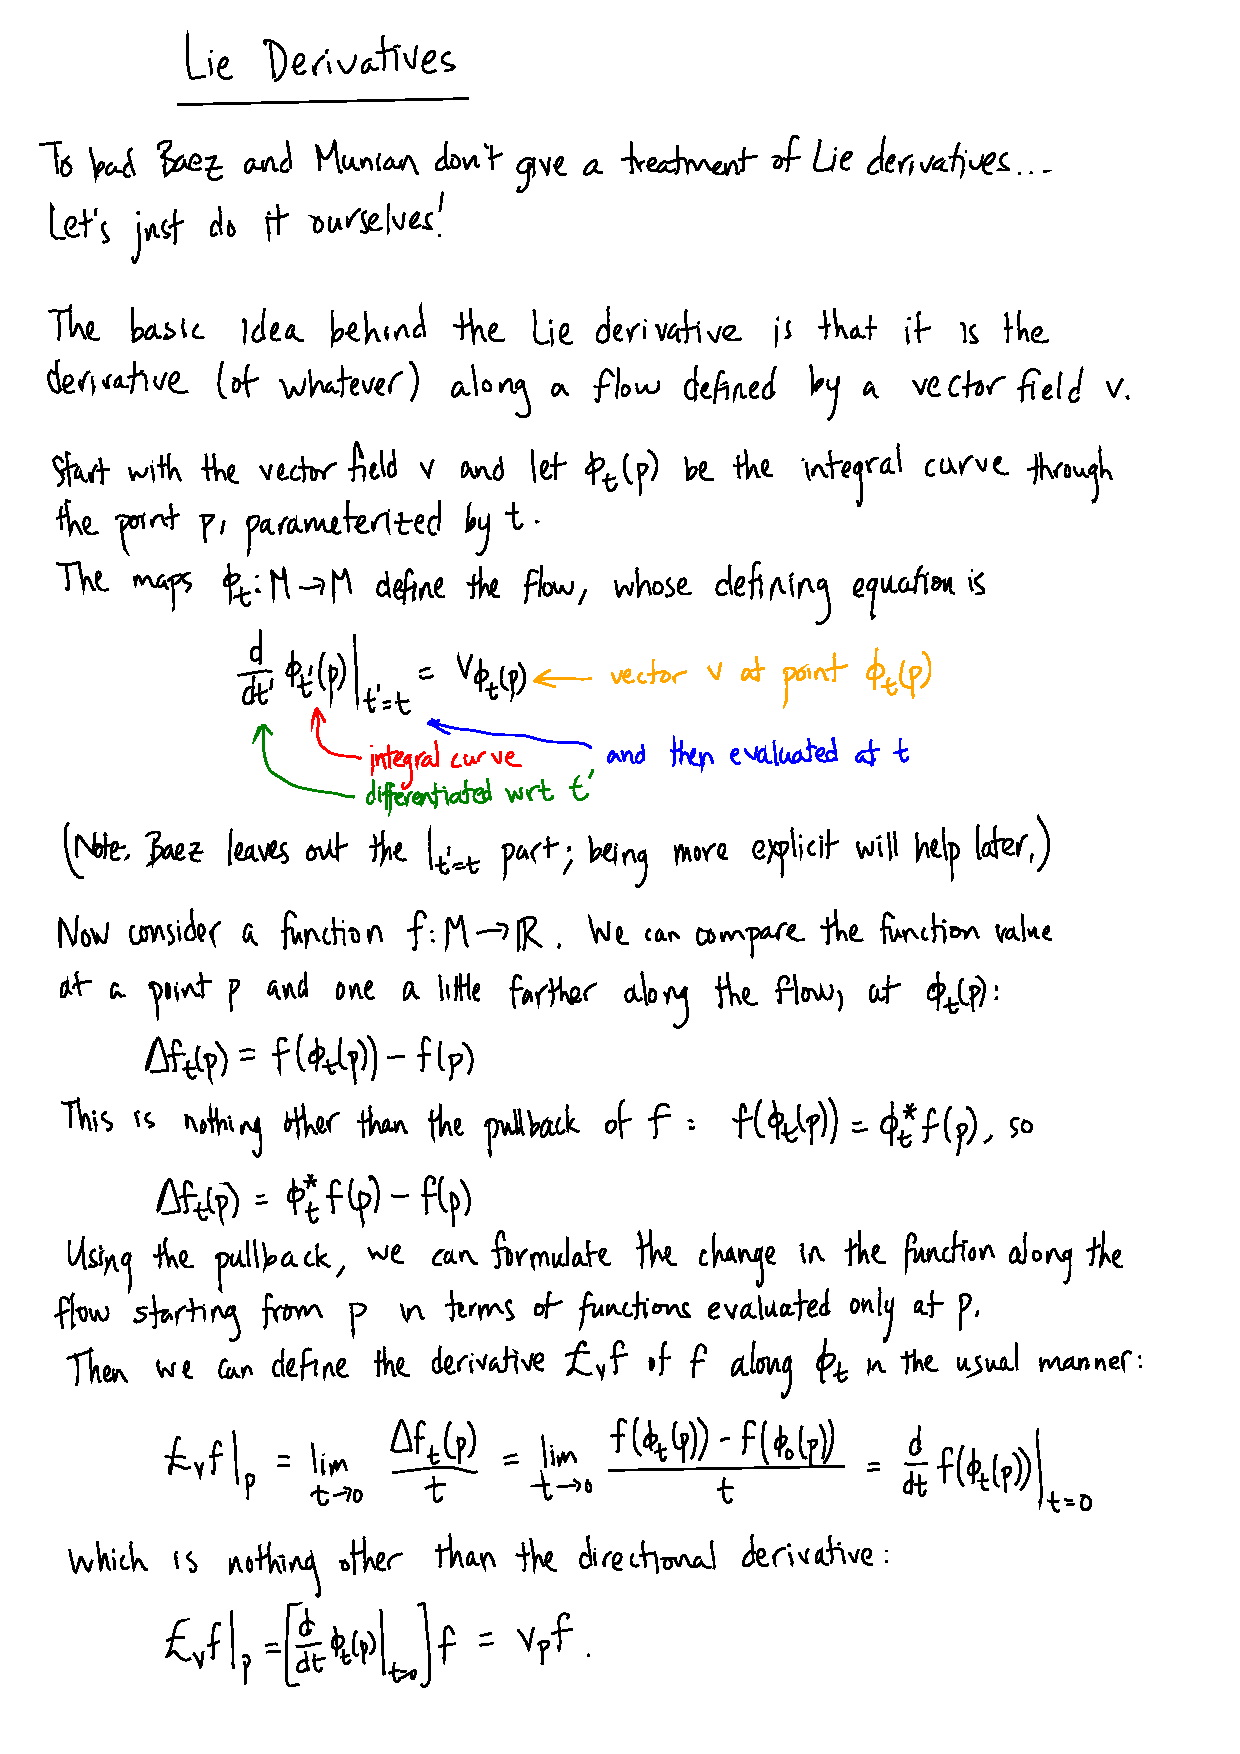
\includepdf[pages=-,addtotoc={1,section,1,The Lie derivative,lie}
]{src/lie.pdf}

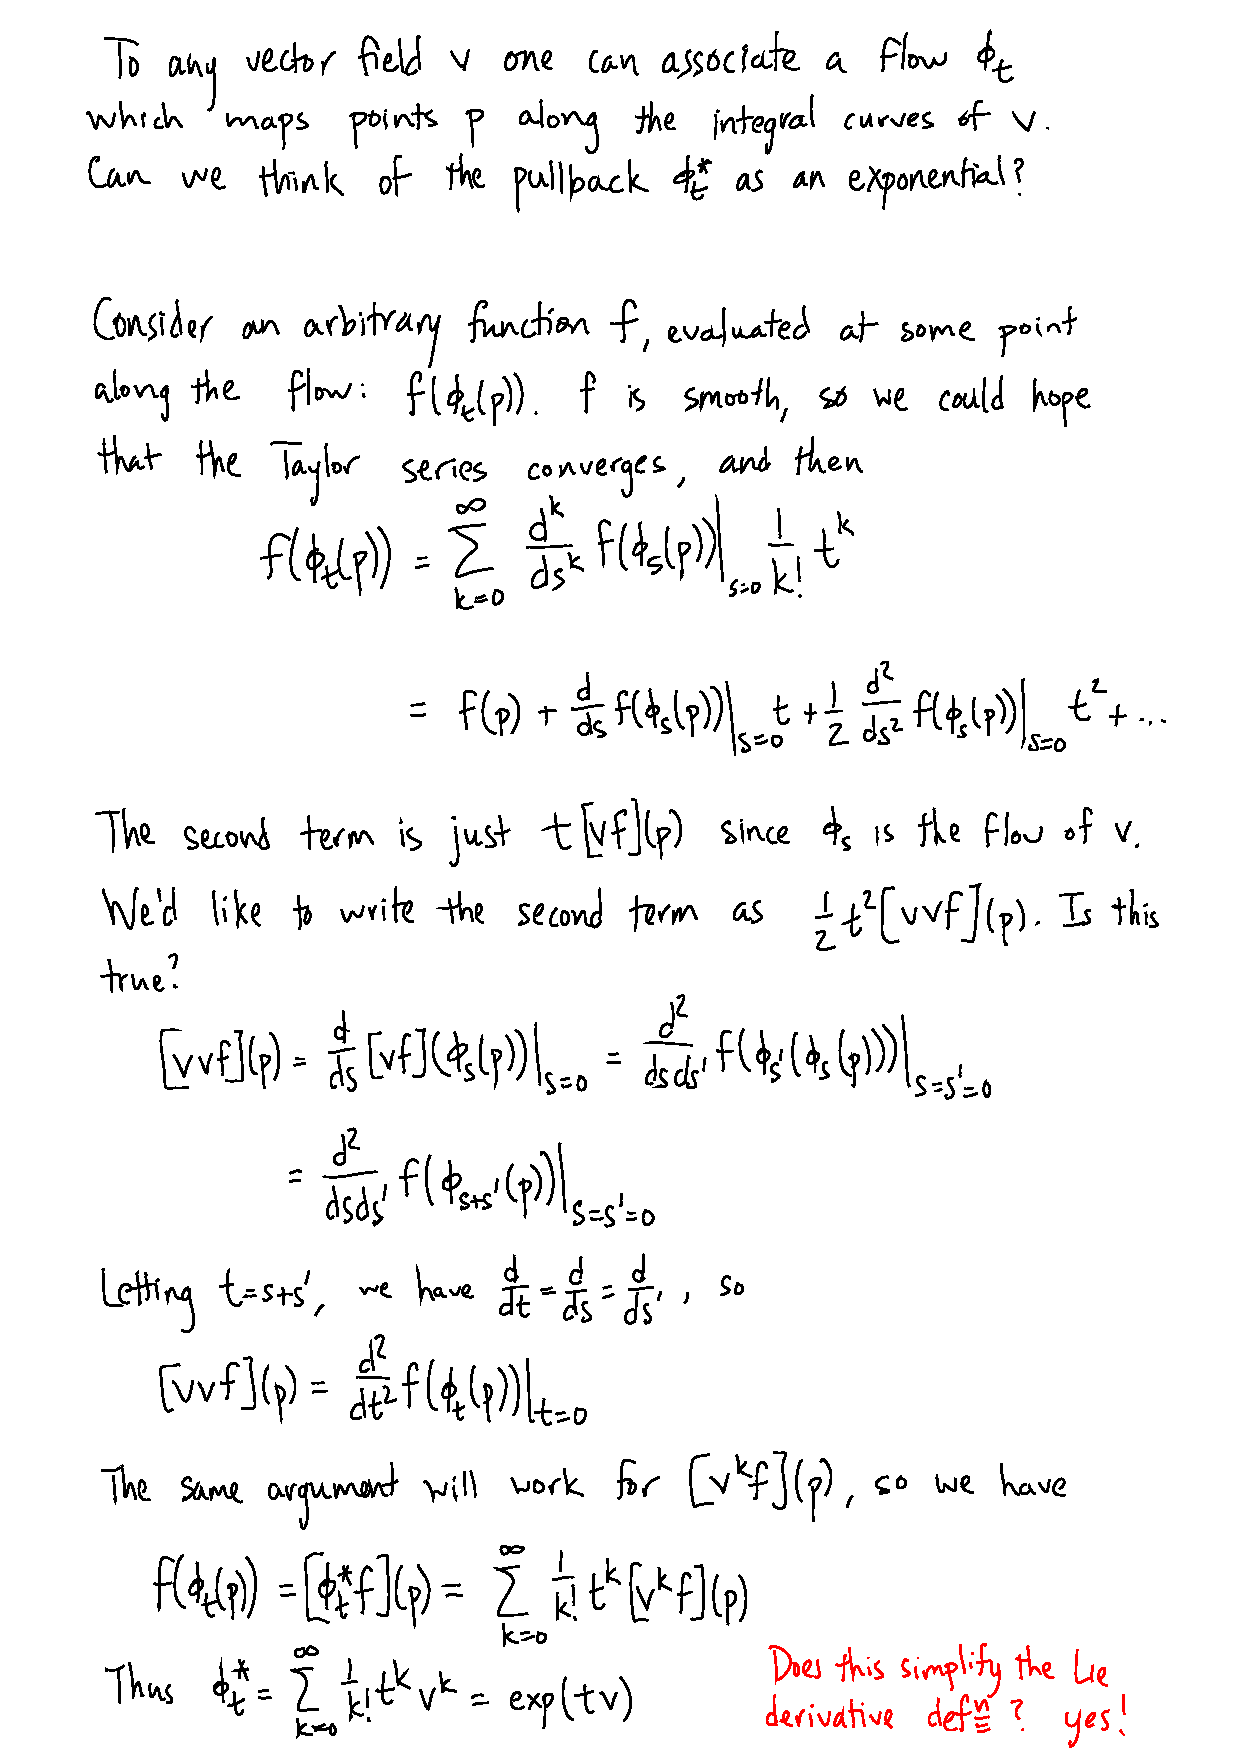
\includepdf[pages=-]{src/expmap.pdf}





\end{document}